%
% CHAPTER - Philosophy of Science
%

\chapterimage{LHC.pdf} % Chapter heading image

\chapter{Analysis of Science}
\label{chap:philosophy-science}

\begin{quote}
\begin{flushright}
\emph{Science may be regarded as the art of data compression.}\\
Li \& Vitányi
\end{flushright}
\end{quote}
\bigskip

{\color{red} TODO: Write this introduction}

In this chapter we will use our theory of nescience to study our current scientific knowledge

We will see how he can approximate the concept of nescience in practice. The concept of surfeit will be based, as it was described in Chaper XX, on the concept of redundancy, and redundancy will be computed in practice based on starndar text compressors.

A historical analyis of the evolution of nescience is also covered in the chapter.

At the end of the chapter we will extend the analysis from individual research topic to research areas, in order to understand 

%
% Section: Describing Current Knowledge
%
\section{Describing Current Knowledge}

According to the theory of nescience, evaluating our current knowledge begins by selecting a specific set of entities we want to understand. Within this framework, universal sets that include every possible entity, whether known or unknown, are not permitted. This restriction arises from the logical paradoxes associated with such sets, including Cantor's theorem, which demonstrates that the set of all subsets has a strictly greater cardinality than the set itself, and Russell's paradox, which involves sets that are not members of themselves (see Section \ref{sec:descriptions_entities}). Therefore, in this chapter, since our objective is to assess the current state of human knowledge, we focus on a finite set composed of entities that are already known and have been studied by science. These entities are suitable for analysis because humanity possesses at least some information about them.

The next step involves identifying the best available encoding of the selected entities as representations, typically composed of data or facts, followed by determining the most accurate descriptions we have, such as models, theories, and laws. In the theory of nescience, we maintain a clear distinction between representations and descriptions because this separation facilitates the discovery of new knowledge: either by improving the representation or by refining the description. However, since our aim here is to evaluate rather than expand our knowledge, we simplify the process by using only descriptions. These descriptions serve both as the representation and the description of an entity (see Section {\color{red} XX}, which explains why descriptions can fulfill both roles). Moreover, we will drop the requirement that these descriptions be computable, since very few scientific descriptions in practice are actually computable. Requiring computability would severely limit the scope of our analysis and exclude a significant portion of scientific knowledge.

For our analysis, we use descriptions derived from the collection of scientific pages from Wikipedia\index{Wikipedia}. Wikipedia is a free, collaborative online encyclopedia launched in 2001 that allows anyone with internet access to create, edit, and update articles on a wide array of topics. It is maintained by a global community of volunteer contributors and aims to provide reliable, neutral, and verifiable information to the public. Several features make Wikipedia particularly suitable for analyzing scientific knowledge: it maintains a transparent version history that tracks content changes over time; supports collaborative validation that reduces individual bias; enforces strict citation requirements to ensure information is verifiable and based on authoritative sources; offers broad and consistent coverage across scientific disciplines; and is dynamically updated to reflect new findings and corrections.

Wikipedia is fundamentally a tertiary source. It compiles and synthesizes information from primary sources, such as firsthand accounts of events or discoveries, and secondary sources, which interpret and evaluate those primary materials. Tertiary sources play a key role in academia by summarizing information that has already been thoroughly discussed and vetted. High-quality Wikipedia articles strive to be comprehensive, covering all major aspects of a topic in appropriate detail while avoiding undue emphasis on minor or peripheral information.

Furthermore, Wikipedia is inherently citational. Every statement included in a Wikipedia article must be supported by a published, reliable, and verifiable source. Original research is not allowed, meaning that novel claims, hypotheses, or breakthroughs must already be published in credible sources such as academic journals or books before being included. Wikipedia also employs a form of peer review, where one or more editors review and suggest improvements to an article. While this process is not anonymous or uniformly applied like traditional academic peer review, it still acts as a quality control mechanism that enhances the coverage, clarity, and accuracy of articles through community oversight.

Wikipedia pages are written in the MediaWiki\index{MediaWiki} Markup Language, a simplified system for formatting text that allows users without technical knowledge of XHTML or CSS to easily edit articles. Before we can analyze the content of a scientific page, it is essential to remove all markup tags and formatting elements to isolate only the meaningful textual information.  To achieve this, we used the Python library \texttt{wikitextparser}\index{Wikitextparser}, which allows us to parse and process the raw wikitext of Wikipedia articles to extract the relevant content. In addition to stripping out the markup, the library was configured to eliminate other non-relevant elements, such as images, references, and lists, which do not contribute directly to our analysis of knowledge.

Wikipedia articles are written in the MediaWiki\index{MediaWiki} Markup Language, a simplified formatting system that allows users without technical expertise to contribute easily. Before we can analyze this content, it is necessary to remove all markup tags and formatting elements to isolate only the meaningful text. To do this, we used the Python library \texttt{wikitextparser}\index{Wikitextparser}, which parses raw wikitext and extracts relevant content. In addition to removing markup, the library was configured to exclude other non-essential elements such as images, references, and lists, which do not directly support our knowledge analysis.

Wikipedia hosts a vast collection of articles covering disciplines such as history, literature, politics, entertainment, and science. Since our goal is to evaluate scientific knowledge specifically, we limited our analysis to articles categorized under the "Science" category. This subset includes topics related to the natural and formal sciences—such as physics, biology, chemistry, and mathematics—ensuring that our study remains aligned with the goal of assessing scientific understanding. We further refined this selection by excluding articles focused on individuals, organizations, awards, lists, portals, and similar metadata-oriented content. This filtering ensures that our analysis includes only those articles centered on scientific concepts, processes, or phenomena.

Both the list of articles and the full content of each article were retrieved directly from Wikipedia using the MediaWiki API\index{MediaWiki API}. This API provides programmatic access to Wikipedia's content, allowing automated queries for page metadata, article text in wikitext format, category information, and revision history. It ensures we are working with the most current and accurate versions of each article while offering a reproducible and efficient method for gathering large-scale data\footnote{The articles analized in this chapter correspond to April 2025.}. A detailed explanation of the entire extraction and preparation process can be found in Appendix \ref{apx:wikipedia}, allowing any interested reader to reproduce the steps and ensure the consistency of the analysis.

%
% Section: Measuring Knowledge
%
\section{Measuring Knowledge}

As mentioned in the previous section, to evaluate our current knowledge in practice, we used the collection of scientific pages from Wikipedia, which we pre-processed to extract the relevant information for our analysis. We focused exclusively on the topic descriptions, treating descriptions and representations as equivalent. In this context, since descriptions and representations are considered the same, the inaccuracy of a topic is effectively zero, leaving miscoding and surfeit as our primary metrics of interest.

\begin{figure}[h]
\centering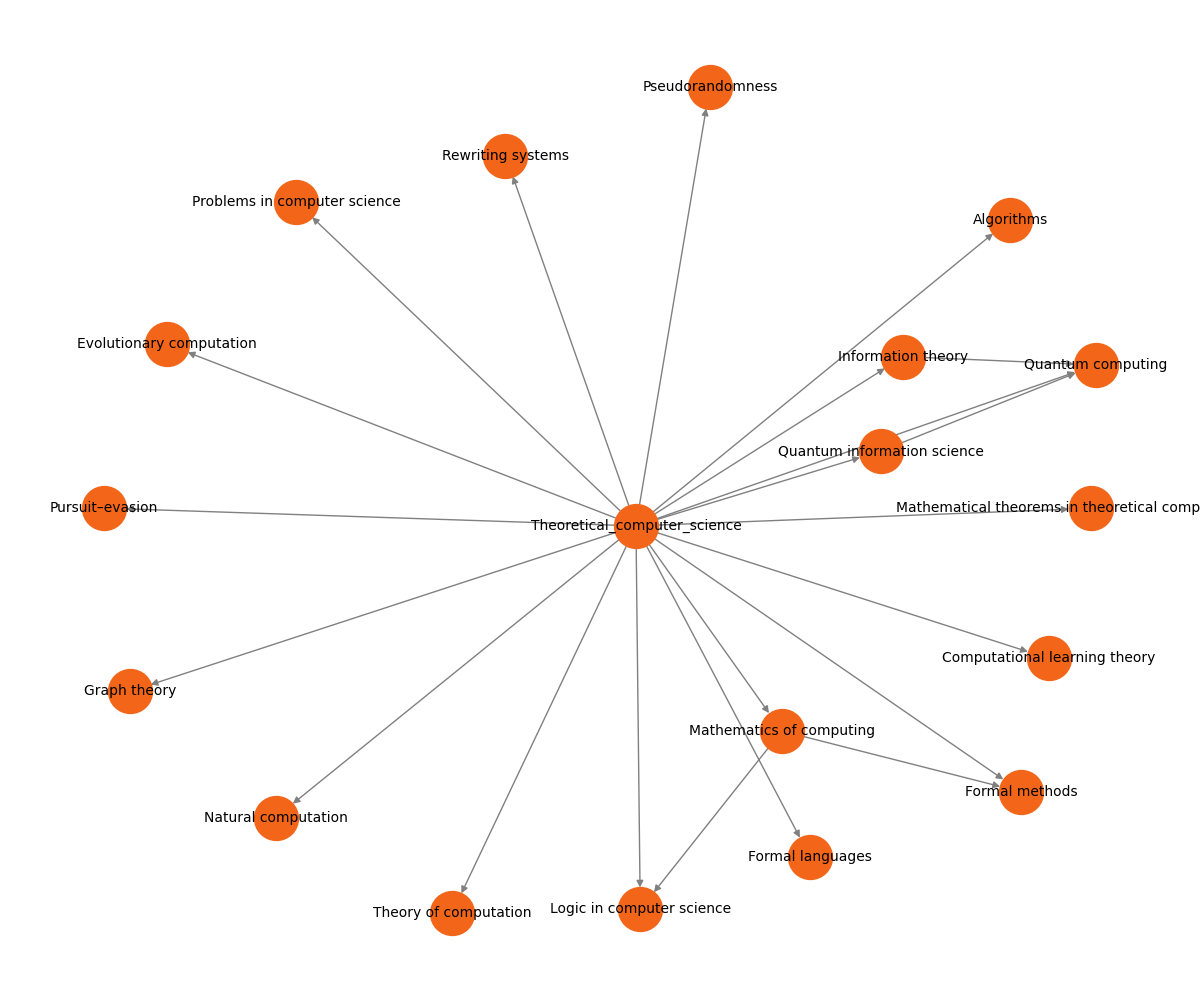
\includegraphics[scale=0.5]{theoretical_computer_science_category_graph}
\caption{\label{fig:theoretical_computer_science_category_graph}Categories in Theoretical Computer Science}
\end{figure}

To demonstrate how our theory can be practically applied to assess the current state of knowledge, we selected a collection of topics listed under the Theoretical Computer Science category on Wikipedia. This includes all pages within the main category, as well as those in its subcategories and their respective subcategories, up to a depth of five levels. Figure \ref{fig:theoretical_computer_science_category_graph} illustrates the Theoretical Computer Science category (Level 1) alongside all its Level 2 subcategories, such as Theory of Computation, Graph Theory, and Logic in Computer Science.

Only pages classified as "GA" have been considered. Articles in the GA class are considered complete, and they have been examined by one or more impartial reviewers. From these list, we have removed pages related to non-relevant topics, such as journals, symposiums, associations, or awards. Additionally, we have removed articles too generic pages (e.g. parallel computing) or pages describing multiple algorihtms (e.g. Tropical cyclone forecasting). For a detailed description of the Wikipedia page preprocessing, please refer to Appendix \ref{apx:wikipedia}.

Only pages classified as "GA" (Good Article) have been considered. GA articles are regarded as complete and have been reviewed by one or more impartial evaluators. From this list, we excluded pages related to non-relevant topics, such as journals, symposiums, associations, or awards. We also removed overly generic articles (e.g., Parallel Computing) and pages describing multiple algorithms (e.g., Tropical Cyclone Forecasting). For a detailed description of the Wikipedia page preprocessing, please refer to Appendix \ref{apx:wikipedia}.

The topics analyzed cover a wide range of areas within theoretical computer science and mathematics. In graph theory, we explored topics such as graph coloring (Greedy coloring), structural properties and special classes (Snark, Perfect graph, Halin graph, Laves graph, Rook's graph, Rado graph, Well-covered graph, Pseudoforest, Component, Unit distance graph, Cop-win graph), graph transformations (Graph homomorphism, Logic of graphs), and graph-based theorems (Steinitz's theorem, De Bruijn–Erdős theorem, Turán's brick factory problem). In algorithms and data structures, we considered classical techniques like Binary search, Selection algorithm, Euclidean algorithm, Fast inverse square root, Farthest-first traversal, Linear probing, Trie, as well as more specialized algorithms such as the Gale–Shapley algorithm, Widest path problem, and data structures like the Cartesian tree. Topics in logic and computational foundations included 2-satisfiability, the Rule of inference, and the BIT predicate. In mathematical methods and theorems, we covered results such as Pick's theorem, Viète's formula, Sylvester–Gallai theorem, Sylvester's sequence, Shapley–Folkman lemma, and the Handshaking lemma. The list also touches on applied mathematics and modeling, through topics like the Dirac delta function, Earth–Moon problem, Tropical cyclone forecast model, Finite subdivision rule, and Network synthesis. Furthermore, in machine learning and computational complexity, we included Reinforcement learning from human feedback and the Small set expansion hypothesis. Finally, some topics address computer science system design and principles, such as the Allocator (C++), Book embedding, Three utilities problem, the Commutative property, and visualization techniques like the Arc diagram. Overall, the list covers a broad spectrum of topics within the area of theoretical computer science, highlighting its diversity and interdisciplinary connections.

\begin{table}
\begin{centering}
\begin{tabular}{|c|c|c|}
\hline 
Algorithm & Analysis of Boolean functions & Automated reasoning \tabularnewline
\hline 
Farthest-first traversal & Gale–Shapley algorithm & Widest path problem \tabularnewline
\hline
Cartesian tree & Viète's formula & Dirac delta function \tabularnewline
\hline
Euclidean algorithm & Fast inverse square root & Rule 184 \tabularnewline
\hline
Binary search & Linear probing & Selection algorithm \tabularnewline
\hline
2-satisfiability & Graph homomorphism & Logic of graphs \tabularnewline
\hline
Steinitz's theorem & De Bruijn–Erdős theorem & Earth–Moon problem \tabularnewline
\hline
Turán's brick factory problem & Laves graph & Rook's graph \tabularnewline
\hline
Snark & Perfect graph & Clique problem \tabularnewline
\hline
Feedback arc set & Euclidean minimum spanning tree & Component \tabularnewline
\hline
Unit distance graph & Halin graph & Cop-win graph \tabularnewline
\hline
Pseudoforest & Well-covered graph & Rado graph \tabularnewline
\hline
Network synthesis & Telephone number (mathematics) & Book embedding \tabularnewline
\hline
Three utilities problem & BIT predicate & Pick's theorem \tabularnewline
\hline
Sylvester–Gallai theorem & RL from human feedback & Finite subdivision rule \tabularnewline
\hline
Sylvester's sequence & Tropical cyclone forecast model & Shapley–Folkman lemma \tabularnewline
\hline
Theil–Sen estimator & Trie & Rule of inference \tabularnewline
\hline
Commutative property & Allocator (C++) & Handshaking lemma \tabularnewline
\hline
\end{tabular}
\par\end{centering}
\caption{\label{tab:Topics-in-theoretical-computer-science}Topics in Theoretical Computer Science}
\end{table}

% Surfeit
\subsection{Surfeit}

In Section \ref{sec:Definition_redundancy}, we introduced the concept of surfeit\index{Surfeit} as a relative measure to quantify the unnecessary effort involved in explaining an entity using a particular description. The surfeit of a description $d$ for a representation $r$ is defined as:
\[
\sigma (d, r) = \frac{ | l(d) - K(r) |}{l(d)}
\]
where $r \in \mathcal{B}^\ast$ and $d \in \mathcal{D}$ is a description of $r$. Intuitively, the less we know about an entity, the longer our description tends to be. As our understanding of the entity improves, we should be able to remove all redundant elements from its description.

In practice, when descriptions and representations are considered equivalent, the concept of surfeit simplifies to:
\[
\rho(d) = 1 - \frac{K(d)}{l(d)}
\]
This is referred to as the redundancy\index{Redundancy} of a description.

The Kolmogorov complexity of the Wikipedia pages was estimated by compressing the raw text. For compression, we used \texttt{bzip2}\index{bzip2}, a free and open-source program based on the Burrows–Wheeler algorithm\index{Burrows–Wheeler algorithm}. bzip2 is commonly used in practice to estimate Kolmogorov complexity because it employs a very large compression buffer. It is well known that if the buffer size is too small, the estimation of a text's Kolmogorov complexity can be significantly distorted. For example, the \texttt{gzip} compressor uses a 32 KB buffer, which is too small for our purposes. In contrast, \texttt{bzip2} offers a buffer size of 900 KB at its highest compression setting (compression level of 9), which is more than sufficient for compressing Wikipedia pages.

Figure \ref{fig:Surfeit-of-Topics} (left) depicts an histogram of the redundancy for the 50 theoretical computer science articles studied. The histogram shows that, once markup and boiler-plate are stripped, redundancy of articles is tightly concentrated between $\approx 0.75$ and $0.82$, peaking near $0.80$. In practical terms, even the clean prose of these pages can typically be shrunk to about three-quarters of its original size, indicating a common stock of recurring phrases, technical jargon, and definitional patterns across the corpus. The scatter plot in figure \ref{fig:Surfeit-of-Topics} (rigth) adds a systematic dimension: redundancy rises by roughly 2–3 percentage points for every additional 10000 characters. Because every file fits inside the single 900 kB block used at \texttt{bzip2}’s highest setting (‐9), block-size effects are neutralised and the only compressor artefacts left—headers and model warm-up—explain at most a few tenths of that increase. The bulk of the slope therefore reflects the prose itself: longer articles increasingly reuse terminology, theorem–proof templates, and explanatory scaffolding, making them intrinsically more compressible. In short, both figures together show that theoretical-computer-science pages share a fairly uniform baseline of linguistic redundancy, and that this redundancy grows gradually with article length because the writing becomes more internally self-similar rather than because of any quirk of the compression tool.

\begin{table}
\begin{centering}
\begin{tabular}{c c}
\includegraphics[width=0.455\textwidth]{Histogram_surfeit}
&
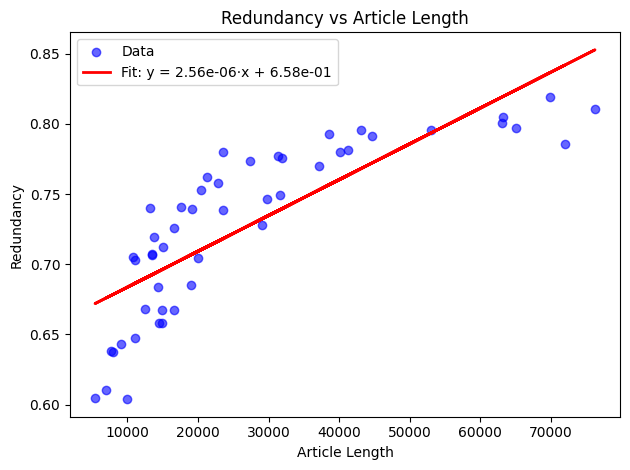
\includegraphics[width=0.5\textwidth]{regression_surfeit}\tabularnewline
\end{tabular}
\par\end{centering}
\caption{\label{fig:Surfeit-of-Topics}Redundancy of Topics}
\end{table}

Table \ref{tab:Higher-redundancy-of-topics} lists the ten topics from Wikipedia within the area of Theoretical Computer Science that exhibit higher redundancy. Each page revolves around a single, well-defined object—a classic algorithm (binary search, Euclidean algorithm, clique problem), a mathematical construct (Dirac delta, Rado graph), or a concise metatheorem (2-SAT, Shapley–Folkman lemma). Pages of this kind inevitably iterate the same symbol palette, definitions, and step-by-step explanations: every subsection restates the object, walks through an example, then re-expresses the same idea in a different formalism (pseudocode, recurrence, proof sketch, code snippet). That self-similar scaffolding gives compressors a wealth of repeated n-grams to exploit, driving redundancy up to 0.79 – 0.82 even after boiler-plate has been stripped. While the list includes some of the longer articles in the corpus (e.g. Dirac delta at 117 kB), it also contains mid-sized pages such as Rado graph (38 kB). In other words, high redundancy is not just a by-product of length; rather, it emerges when a compact conceptual core is expanded through multiple parallel presentations (history, intuition, formal statement, variations, applications, proof, pseudocode).

\begin{table}
\begin{centering}
\begin{tabular}{|c|c|c|c|}
\hline 
Topic & Redundancy & Page Length & Length Compressed \tabularnewline
\hline 
\hline 
Dirac delta function & 0.821 & 117121 & 20969 \tabularnewline
\hline
Binary search & 0.819 & 69838 & 12634 \tabularnewline
\hline
Euclidean algorithm & 0.811 & 113242 & 21455 \tabularnewline
\hline
2-satisfiability & 0.811 & 76225 & 14442 \tabularnewline
\hline
Shapley–Folkman lemma & 0.805 & 63172 & 12323 \tabularnewline
\hline
Clique problem & 0.801 & 63125 & 12574 \tabularnewline
\hline
RL from human feedback & 0.797 & 64981 & 13160 \tabularnewline
\hline
Book embedding & 0.796 & 53046 & 10831 \tabularnewline
\hline
Rule of inference & 0.795 & 43158 & 8826 \tabularnewline
\hline
Rado graph & 0.793 & 38626 & 7989 \tabularnewline
\hline 
\end{tabular}
\par\end{centering}
\caption{\label{tab:Higher-redundancy-of-topics}Topics with higher redundancy}
\end{table}

Table \ref{tab:Lower-redundancy-of-topics} lists the ten topics that exhibit lower redundancy. These articles sit in the low–redundancy tail (between 0.60 and 0.67) differ from the high-redundancy ones in both size and content mix. (i)  Every entry is under 17 kB—well below the corpus median. Because bzip2’s fixed header and model “warm-up” overhead account for a larger share of such small files, their redundancy starts a few percentage points lower even before content is considered. This matches the positive slope in the scatter-plot: shorter pages naturally cluster toward the left-hand foot of the trend line. (ii) Many of these topics centre on a single formula, sequence, or code idiom (e.g. Viète’s formula, Sylvester’s sequence, Allocator). They pack unique symbols, numeric constants and one-off identifiers that appear only once or twice, so compressors see far fewer repeated n-grams than in algorithm-walk-through articles. Others, such as "Tropical cyclone forecast model" and "Finite subdivision rule", read more like concise surveys, stringing together disparate subtopics rather than iterating one core definition from multiple angles; that heterogeneity also suppresses repetition.

Together, the list illustrates the floor of the redundancy spectrum: pages that are (i) short enough for compression overhead to matter and (ii) information-dense or eclectic enough to avoid recycling the same prose patterns never reach the 0.70–0.80 plateau seen elsewhere.  Their position reinforces the earlier finding that rising redundancy with length is not merely a compressor artefact; it also depends on how much authors reuse terminology and explanatory scaffolding as an article grows.

\begin{table}
\begin{centering}
\begin{tabular}{|c|c|c|c|}
\hline 
Topic & Redundancy & Page Length & Length Compressed \tabularnewline
\hline 
\hline 
Tropical cyclone forecast model & 0.667 & 16675 & 5550 \tabularnewline
\hline
Allocator (C++) & 0.658 & 14887 & 5085 \tabularnewline
\hline
Finite subdivision rule & 0.658 & 14416 & 4933 \tabularnewline
\hline
Snark (graph theory) & 0.648 & 11020 & 3882 \tabularnewline
\hline
Theil–Sen estimator & 0.643 & 9171 & 3275 \tabularnewline
\hline
Earth–Moon problem & 0.638 & 7640 & 2762 \tabularnewline
\hline
Halin graph & 0.637 & 7953 & 2885 \tabularnewline
\hline
Viète's formula & 0.61 & 7016 & 2733 \tabularnewline
\hline
Turán's brick factory problem & 0.605 & 5427 & 2146 \tabularnewline
\hline
Sylvester's sequence & 0.604 & 9994 & 3960 \tabularnewline
\hline 
\end{tabular}
\par\end{centering}
\caption{\label{tab:Lower-redundancy-of-topics}Topics with Lower redundancy}
\end{table}

% Subsection: Inaccuracy
\subsection{Inaccuracy}

Inaccuracy serves as the second metric in assessing our understanding of a research entity. The underlying idea is that the more accurate our model, the better our understanding of the entity. Formally, we calculate the inaccuracy of a description $d$ as the normalized information distance between the original representation $r$ and the output representation $r'$ generated by our description $d$. That is, inaccuracy is quantified as the length of the smallest computer program capable of correcting the erroneous output of our model.

Inaccuracy, serving as the second gauge to measure our comprehension of a research entity, is based on the principle that the more precise our model, the better our grasp of the entity. Formally, the inaccuracy of a description $d$ is computed as the normalized information distance between the original representation $r$ and the output representation $r'$ generated by the description $d$. Thus, inaccuracy is assessed as the extent of the smallest computer program that can rectify the incorrect output of our model.

Inaccuracy evaluates how well the output of our description aligns with the selected representation encoding the entity. However, this representation could be flawed itself, as discussed in the preceding chapter. Inaccuracy focuses solely on the description $d$, neglecting the potential miscoding within the representation $r$. Furthermore, even though it doesn't require an oracle, inaccuracy cannot be calculated for every case, so it needs to be estimated in practical situations, as we will explore in Part III of this book.

Let us consider $r \in \mathcal{B}^\ast$ as a representation, and $d \in \mathcal{D}$ as a description, where $d = \langle TM, a \rangle$. We then define the \emph{inaccuracy} of the description $d$ with respect to the representation $r$, denoted as $\iota(d, r)$, according to the following formula:
\[
\iota(d, r) = \frac{ \max\{ K \left(r \mid \delta(d) \right), K \left( \delta(d) \mid r \right) \} } { \max\{ K(r), K \left(\delta(d) \right) \} }
\]
Intuitively, accuracy measures the difficulty in converting an incorrect representation $r'$ produced by a desription $d$ into the original representation $r$. In essence, this involves the computation of the normalized information distance between $r'$ and $r$.

In practice, and in the particular case of descriptions based on the scientific articles of Wikipedia, we cannot apply this definition, because an article of Wikipedia is not a Turing machine that produces a string based output.

Figure \ref{fig:Nescience-of-Topics} left depicts a histogram showing the inaccuracy of the analyzed topics, and right side shows a scatterplot of the article lenghts vs. the length of the correspondign talk pages, toghether with a regression line fitted to the data. The two plots suggest that, within this sample of good-quality theoretical computer science pages, talk pages chatter is generally modest and becomes proportionally smaller as articles grow. Inaccuracy, approximated as talk / (article + talk), is highly right-skewed.  Roughly half the pages fall below 0.05 and more than three-quarters below 0.15, meaning their talk pages contain at most one word of discussion for every six to twenty words of main-text content.  Only a small tail of articles pushes beyond 0.40, indicating a handful of topics that still attract extensive debate or revision despite their “good” label. In the scatter plot we can observe that the best-fit line ( $y \approx -2.44 \times 10^{-6} \dot length + 0.271$ ) slopes downward, so predicted inaccuracy drops from about 0.27 for a 0-length stub to $\approx 0.10$ at 70 kB.  Empirically, short articles (< 15 kB) show the widest spread—from virtually no talk to talk pages two-thirds the size of the article—whereas long articles (> 50 kB) cluster below 0.15 with only rare outliers.  In other words, once an article expands to tens of thousands of characters, the relative volume of unresolved discussion shrinks, suggesting that length correlates with maturity and consensus. Taken together, the figures imply that most good theoretical-CS pages are comparatively settled, that the few contentious ones are disproportionately short, and that growing an article tends to absorb or resolve the issues reflected on its talk page rather than magnifying them.

\begin{table}
\begin{centering}
\begin{tabular}{c c}
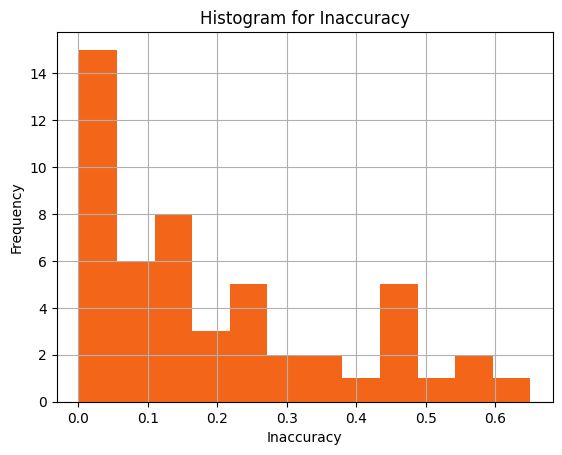
\includegraphics[width=0.455\textwidth]{Histogram_inaccuracy}
&
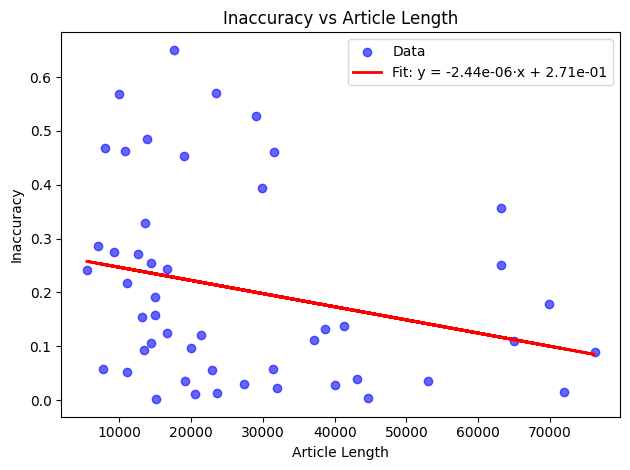
\includegraphics[width=0.5\textwidth]{regression_inaccuracy}\tabularnewline
\end{tabular}
\par\end{centering}
\caption{\label{fig:Inaccuracy-of-Topics}Inaccuracy of Topics}
\end{table}

Table \ref{tab:Lower-nescience-of-topics} lists topics exhibiting the lowest levels of nescience. The topics with the lowest inaccuracy values ($\leq 0.04$) look like settled science. They cover classical, mathematically-rigorous results—matching algorithms (Gale–Shapley), structural graph properties (perfect graphs, Steinitz’s theorem), and well-studied data-structures or routing primitives (Cartesian tree, widest-path problem). For such topics there is little room for interpretive dispute: statements are either formally correct or not, and once a clean exposition is in place subsequent editors rarely need lengthy back-and-forth. That is why some talk pages are only a few dozen words long (25 for Gale–Shapley) even when the article itself spans tens of kilobytes. Length alone does not guarantee a quiet talk page—the list includes both mid-sized texts ($\approx 20$ kB) and the 72 kB Network synthesis article—yet all of them keep the ratio of discussion to content below 4\%. Where talk does appear (e.g. 1 989 words for Book embedding or 1 145 for Steinitz’s theorem) it is still dwarfed by the main text, implying that open issues tend to be minor wording tweaks, sourcing details, or peripheral expansions rather than fundamental disagreements. In short, low-inaccuracy articles are those whose subject matter is uncontroversial, formally locked-down, and already presented in a stable, comprehensive fashion, leaving editors with little need for ongoing debate.

\begin{table}
\begin{centering}
\begin{tabular}{|c|c|c|c|}
\hline 
Topic & Inaccuracy & Article length & Talk length \tabularnewline
\hline 
\hline
Gale–Shapley algorithm & 0.001656 & 15072 & 25 \tabularnewline
\hline
Perfect graph & 0.004412 & 44683 & 198 \tabularnewline
\hline
Unit distance graph & 0.012203 & 20479 & 253 \tabularnewline
\hline
Rook's graph & 0.013267 & 23576 & 317 \tabularnewline
\hline
Network synthesis & 0.014493 & 71945 & 1058 \tabularnewline
\hline
Logic of graphs & 0.022260 & 31933 & 727 \tabularnewline
\hline
Steinitz's theorem & 0.027765 & 40094 & 1145 \tabularnewline
\hline
Cartesian tree & 0.030849 & 27395 & 872 \tabularnewline
\hline
Widest path problem & 0.035644 & 19128 & 707 \tabularnewline
\hline
Book embedding & 0.036141 & 53046 & 1989 \tabularnewline
\hline
\end{tabular}
\par\end{centering}
\caption{\label{tab:Lower-inaccuracy-of-topics}Topics with lower inaccuracy}
\end{table}

Finally, Table \ref{tab:Higher-inaccuracy-of-topics} lists the topics with the highest nescience values. The articles with the highest inaccuracy scores are not necessarily the most error-ridden; rather, they are the ones whose talk pages have become arenas for protracted discussion because their subjects invite disagreement or continual refinement—foundational concepts like the commutative property and tries that draw many first-time editors, folklore-tinged algorithms such as the fast inverse square root, or theorems and graph classes (e.g., Sylvester–Gallai, pseudoforests, Halin graphs) that have multiple equivalent statements, proofs, or naming conventions.  In every case the talk page approaches or even exceeds the size of the main text, so anywhere from 40\% to 65\% of the combined bytes are debate rather than exposition; this ratio is amplified by the fact that most of these articles are relatively short ($\approx 10–30$ kB), meaning even modest amounts of conversation loom large.  Together they illustrate that a high inaccuracy score chiefly signals ongoing editorial contention—about scope, presentation order, historical credit, or performance claims—rather than a simple lack of factual correctness, and that such contention is most pronounced where definitions are ambiguous, folklore collides with formalism, or broad audiences repeatedly revisit basic material.

\begin{table}
\begin{centering}
\begin{tabular}{|c|c|c|c|}
\hline 
Topic & Inaccuracy & Article length & Talk length \tabularnewline
\hline 
\hline 
Sylvester–Gallai theorem & 0.394610 & 29810 & 19431 \tabularnewline
\hline
Pseudoforest & 0.454130 & 18999 & 15806 \tabularnewline
\hline
Selection algorithm & 0.461374 & 31578 & 27049 \tabularnewline
\hline
BIT predicate & 0.463016 & 10817 & 9327 \tabularnewline
\hline
Halin graph & 0.467671 & 7953 & 6987 \tabularnewline
\hline
Three utilities problem & 0.485948 & 13846 & 13089 \tabularnewline
\hline
Fast inverse square root & 0.528723 & 29001 & 32536 \tabularnewline
\hline
Sylvester's sequence & 0.567808 & 9994 & 13130 \tabularnewline
\hline
Trie & 0.570980 & 23503 & 31280 \tabularnewline
\hline
Commutative property & 0.650826 & 17583 & 32773 \tabularnewline
\hline 
\end{tabular}
\par\end{centering}
\caption{\label{tab:Higher-inaccuracy-of-topics}Topics with higher inaccuracy}
\end{table}

% Subsection: Nescience
\subsection{Nescience}

According to the theory of nescience, our understanding of an entity should be based on the quality of the description used to explain it. In Chapter \ref{chap:Nescience}, we introduced a quantitative measure of our ignorance regarding a research entity. This measure depends on the miscoding of a string-based representation of the entity, as well as the inaccuracy and surfeit of the model describing this representation. Ideally, we seek representations and descriptions that simultaneously minimize these three aspects.

In practical terms, particularly when entities correspond to topics covered by scientific Wikipedia pages, we consider only the surfeit and inaccuracy of a description. In this scenario, the representation of a topic coincides with its description, rendering the computation of miscoding irrelevant.

To address the multi-objective optimization problem posed by nescience, we apply a global criterion approach (see Section \ref{sub:multiobjective_global_criterion}). This method solves multi-objective optimization problems by minimizing the distance between a chosen reference point and the feasible region of the objective space. We select the origin vector $(0, 0)$ as our reference point. The distance metric used will be the harmonic mean of surfeit and inaccuracy, defined as:
\[
\frac{2}{ \iota(d, r)^{-1} + \sigma(d, r)^{-1} }
\]
As described in previous sections, surfeit is approximated by the redundancy of the topic's description (the Wikipedia page), while inaccuracy is estimated by the length of the corresponding Talk page.

As it was explained in Section {\color{red} XX}, since we are using a decision maker to compute nescience based on redundancy and inaccuracy, and since these quantities do not have the same scale, it is highly convenient to apply the following additional transformation to them:
\[
\mu_{t}^{,}=\frac{\mu_{t}-\min(\mu)}{\max(\mu)-\min(\mu)}
\]
where $\mu_t$ refers to the considered metric (nescience, relevance, ...). 

Figure \ref{fig:Nescience-of-Topics} left depicts a histogram showing the nescience levels of the analyzed topics, and right side shows a scatterplot of the article lenghts vs. the nescience, toghether with a regression line fitted to the data. The two panels paint a mixed picture of how much “unknown-ness” remains in these 50 “good” theoretical-CS articles once both redundancy (compressibility of the prose) and inaccuracy (relative size of the talk page) are factored in. Histogram — a long, uneven tail. Roughly one-third of the articles cluster below nescience $\approx 0.10$, meaning they are simultaneously concise (low redundancy) and largely uncontested (little talk).  Frequency then stays fairly flat through the 0.15 – 0.35 band and drops again, before a second bump appears between 0.60 and 0.75.  That small peak corresponds to pages that are both highly repetitive and heavily debated—the same ones that topped the earlier redundancy and inaccuracy lists.  In short, while many good-class pages are well understood, a non-trivial minority still exhibits a pronounced knowledge gap. Scatter plot — almost length-neutral. The best-fit line rises only 0.007 points for every additional 10 000 characters (slope $\approx 7.5 \times 10^{-7}$), so article length alone is not a strong predictor of nescience.  Short pages can swing from near-zero to 0.7, depending on how contentious they are, whereas long pages (> 50 kB) compress more (pushing nescience up) but also attract proportionally less talk (pushing it down), leaving them parked in a mid-range around 0.25–0.35.  The gentle upward tilt therefore reflects the fact that redundancy grows with length a bit faster than inaccuracy falls, but the wide vertical spread shows that editorial stability—rather than size—is the decisive factor. Overall, “good” status keeps most theoretical-CS articles in a low-to-moderate nescience zone, yet about a quarter of them still suffer from enough repetition and unresolved discussion to signal that our coverage of those topics remains less mature than the label might suggest.

\begin{table}
\begin{centering}
\begin{tabular}{c c}
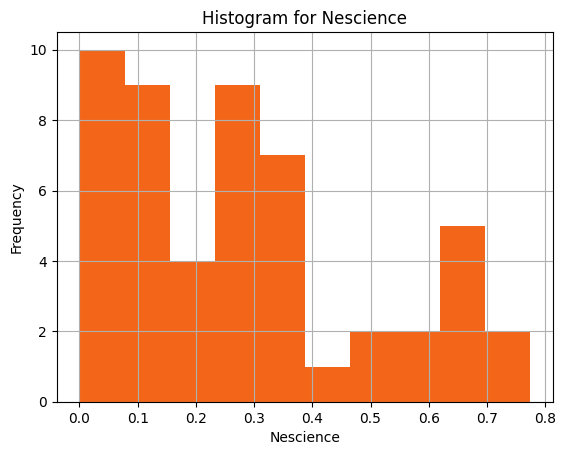
\includegraphics[width=0.455\textwidth]{Histogram_nescience}
&
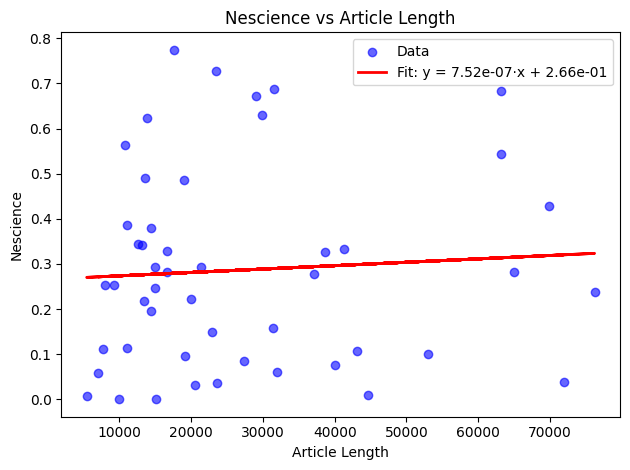
\includegraphics[width=0.5\textwidth]{regression_nescience}\tabularnewline
\end{tabular}
\par\end{centering}
\caption{\label{fig:Nescience-of-Topics}Nescience of Topics}
\end{table}

Table \ref{tab:Lower-nescience-of-topics} lists topics exhibiting the lowest levels of nescience. The articles that score best on the nescience metric fall into two complementary archetypes, each driving the harmonic mean down by making one of the two ingredients—redundancy or inaccuracy—almost vanish.  The first archetype is epitomised by "Sylvester ’s sequence" and "Turán’s brick-factory problem": they are short, information-dense pages whose prose compresses poorly (normalized redundancy $\approx 0$), so even a rather lively talk page cannot lift their nescience above zero.  The second archetype—illustrated by "Gale–Shapley algorithm", "Perfect graph", "Network synthesis", and several other graph-theoretic topics—shows the opposite pattern: their text is highly repetitive (normalized redundancy $\approx 0.8–0.86$), but the talk pages are almost silent, so inaccuracy is near zero and the harmonic mean again collapses.  Taken together, the list reveals that low lack-of-knowledge can arise either from concise, debate-heavy but non-redundant expositions or from long, internally repetitive but well-settled treatments; what matters for nescience is that at least one dimension of uncertainty is squeezed to the floor.

\begin{table}
\begin{centering}
\begin{tabular}{|c|c|c|c|}
\hline 
Topic & Nescience & Norm. Inaccuracy & Norm. Redundancy \tabularnewline
\hline 
\hline
Sylvester's sequence & 0.000000 & 0.872117 & 0.000000 \tabularnewline
\hline
Gale–Shapley algorithm & 0.000000 & 0.000000 & 0.499166 \tabularnewline
\hline
Turán's brick factory problem & 0.007362 & 0.370945 & 0.003718 \tabularnewline
\hline
Perfect graph & 0.008448 & 0.004245 & 0.864084 \tabularnewline
\hline
Unit distance graph & 0.031744 & 0.016248 & 0.686717 \tabularnewline
\hline
Rook's graph & 0.035003 & 0.017887 & 0.812327 \tabularnewline
\hline
Network synthesis & 0.038635 & 0.019774 & 0.836612 \tabularnewline
\hline
Viète's formula & 0.057626 & 0.437415 & 0.030845 \tabularnewline
\hline
Logic of graphs & 0.061030 & 0.031738 & 0.791546 \tabularnewline
\hline
Steinitz's theorem & 0.076638 & 0.040219 & 0.811139 \tabularnewline
\hline 
\end{tabular}
\par\end{centering}
\caption{\label{tab:Lower-nescience-of-topics}Topics with lower nescience}
\end{table}

Finally, Table Finally, Table \ref{tab:Higher-nescience-of-topics} lists the topics with the highest nescience values. The upper tail of the nescience scale is populated by pages that score high on both axes at once —they are repetitive and heavily debated—so the harmonic mean refuses to average the trouble away.  Half of the list ("BIT predicate", "Three-utilities problem", "Fast inverse square root", "Selection algorithm", "Trie", "Commutative property") shows normalized-inaccuracy $\geq 0.70$, signalling talk pages that rival the article in size; the same set attracts a steady stream of newcomers or folklore-laden claims, which keeps discussion alive.  The other half ("Shapley–Folkman lemma", "Clique problem", "Sylvester–Gallai theorem", "Farthest-first traversal") earns its place chiefly through very high redundancy ($\approx 0.90$ in the case of the clique problem), reflecting articles that restate definitions, proofs and examples in multiple near-duplicate forms.  In every case the other dimension is still uncomfortably large ($\geq 0.38$), so neither trimming repetition nor settling open talk-page issues alone would be enough to pull these topics out of the danger zone.  In short, high-nescience entries are those where unresolved editorial contention co-exists with a self-similar writing style—pages that simultaneously need consensus-building and structural tightening before they can be considered well understood.

\begin{table}
\begin{centering}
\begin{tabular}{|c|c|c|c|}
\hline 
Topic & Nescience & Norm. Inaccuracy & Norm. Redundancy \tabularnewline
\hline 
\hline
Farthest-first traversal & 0.490109 & 0.505215 & 0.475880 \tabularnewline
\hline
Shapley–Folkman lemma & 0.543853 & 0.384947 & 0.926181 \tabularnewline
\hline
BIT predicate & 0.562673 & 0.710692 & 0.465683 \tabularnewline
\hline
Three utilities problem & 0.622535 & 0.746017 & 0.534125 \tabularnewline
\hline
Sylvester–Gallai theorem & 0.629670 & 0.605318 & 0.656063 \tabularnewline
\hline
Fast inverse square root & 0.671295 & 0.811908 & 0.572197 \tabularnewline
\hline
Clique problem & 0.683333 & 0.548081 & 0.907206 \tabularnewline
\hline
Selection algorithm & 0.688247 & 0.708163 & 0.669420 \tabularnewline
\hline
Trie & 0.727080 & 0.877003 & 0.620932 \tabularnewline
\hline
Commutative property & 0.774591 & 1.000000 & 0.632109 \tabularnewline
\hline 
\end{tabular}
\par\end{centering}
\caption{\label{tab:Higher-nescience-of-topics}Topics with higher nescience}
\end{table}

\subsection{Conclusion}

Across the 50 “good-class” Wikipedia pages in theoretical computer science, our indicators tell a nuanced story about what the encyclopaedia can reveal—and obscure—about collective understanding.  Talk-page activity, captured by our inaccuracy ratio, does a credible job of flagging articles whose content is still contested: pages with minimal discussion almost always cover settled, formally unambiguous material, whereas those whose talk pages rival the main text correspond to concepts riddled with naming ambiguity, folklore or pedagogical disagreement. Redundancy, distilled from compression ratios after stripping boiler-plate, complements this view by signalling how tightly authors have distilled the topic: low values align with concise, information-dense expositions, while high values mark articles that re-iterate definitions, proofs and code snippets in multiple guises.  Each metric thus illuminates a different facet—editorial consensus on one side, stylistic efficiency on the other—yet neither by itself captures “knowledge quality” outright.

Their harmonic mean, which we dubbed nescience, succeeds as a triage tool because it punishes a topic the moment either dimension becomes extreme. Articles that are both verbose and hotly debated—such as those on the fast inverse square root or the clique problem—cluster at the high end, clearly pointing to areas where Wikipedia’s coverage remains unsettled. Conversely, pages with either crisp, irredundant prose or near-empty talk pages sink to the bottom, reflecting mature, well-understood subjects like the Gale–Shapley algorithm or perfect graphs. In that sense, nescience offers a practical snapshot of our residual ignorance as reflected in the encyclopaedia: it reliably highlights where clarification, consolidation or further research are still needed, even if it cannot, on its own, disentangle whether the root cause is factual dispute, pedagogical complexity, or simple editorial neglect.

%
% Section: Measuring Resarch Areas
%

\section{Measuring Research Areas}

In this section, we evaluate the nescience of entire research areas rather than individual topics, measuring how much knowledge each discipline encompasses. We examined all English‑language “good‑class” articles in six broad disciplines (biology, chemistry, mathematics, philosophy, physics, and psychology) comprising roughly 600 pages (see Table \ref{tab:num_topics_per_area}). For each discipline, we assessed three metrics: inaccuracy, redundancy, and nescience.

\begin{table}
\begin{centering}
\begin{tabular}{|c|c|}
\hline 
Area & Num. Topics \tabularnewline
\hline 
\hline
Biology & 214 \tabularnewline
\hline
Philosophy & 33 \tabularnewline
\hline
Psychology & 44 \tabularnewline
\hline
Mathematics & 127 \tabularnewline
\hline
Chemistry & 138 \tabularnewline
\hline
Physics & 52 \tabularnewline
\hline
\end{tabular}
\par\end{centering}
\caption{\label{tab:num_topics_per_area}Number of topics analyzed per area}
\end{table}

Wikipedia organizes articles into categories by topic to simplify navigation and discovery. Rather than a strict hierarchy, categories form an interconnected network: each category can have multiple subcategories, and a subcategory may belong to multiple parent categories. Editors avoid circular links, where a category would indirectly include itself through its descendants. Conceptually, this structure resembles a partially ordered set\index{Partially ordered set} in mathematics and computer science, and it allows diverse classification schemes to coexist within a unified framework. When one category clearly falls under another, it is designated as a subcategory to preserve a logical “is‑a” relationship. Articles are typically placed only in their most specific relevant category to avoid redundancy. For example, the article on Claude Shannon appears in “Category:American information theorists,” not directly under the broader “Category:Mathematicians.”

The top level of Wikipedia’s category system is “Category:Contents,” which has no parent. From there, the path we have used proceeds as: Contents → Articles → Main topic classification → Academic disciplines → Science → Branches of Science (Applied Sciences, Formal Sciences, Natural Sciences, Social Sciences). Our analysis focuses on five scientific areas: Mathematics, which falls under Formal Sciences; Biology, classified within Life Sciences under Natural Sciences; Physics and Chemistry, both part of Physical Sciences in the Natural Sciences; and Psychology, included in Social Sciences. We also analyze Philosophy, categorized under Humanities within Academic disciplines. These selections ensure comprehensive coverage of both theoretical and empirical fields.

\begin{figure}[h]
\centering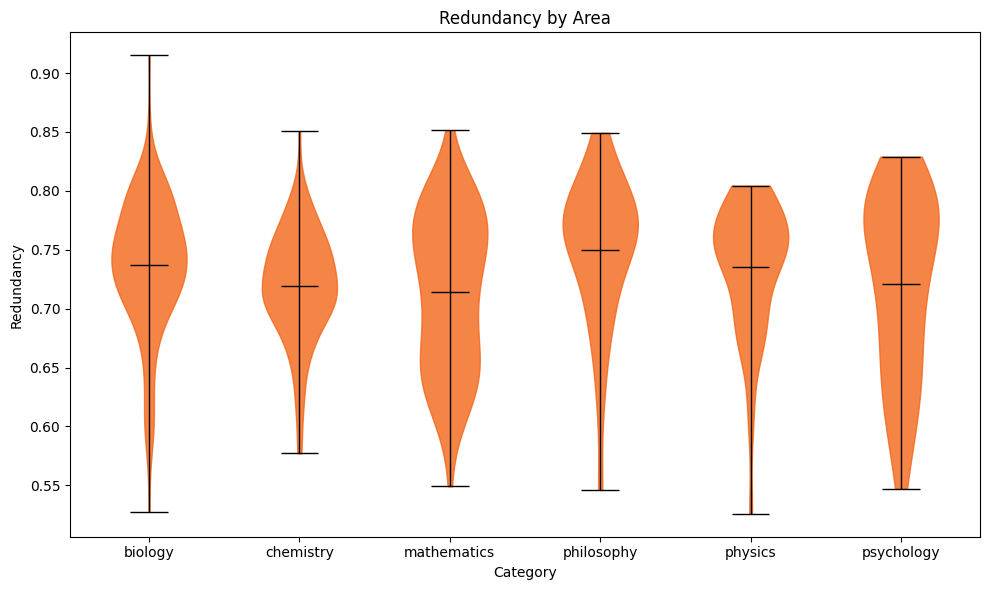
\includegraphics[scale=0.5]{redundancy_by_area}
\caption{\label{fig:redundancy-by-area}Redundancy by Area}
\end{figure}
 
First, we looked at redundancy (see Figure \ref{fig:redundancy-by-area}), which shows how much an article repeats itself. We took out templates, lists, and other markup, then compressed each page using bzip2 at its highest setting. Pages with more repeated text stay larger after compression. We found that most good articles in every field fall in a redundancy range of about 0.70 to 0.80, so they repeat text at similar rates. Biology had the widest range, from about 0.52 up to over 0.90, meaning some articles are very concise while others include many standard sections. Chemistry was the most consistent group, clustering around 0.72, possibly because of regular naming rules and reaction sections. Mathematics, philosophy, physics, and psychology were all in the middle, with medians near 0.75 but small differences in spread. For example, math and philosophy pages sometimes repeat proofs or arguments, raising their upper range, while psychology has some short experiment-focused articles. Physics looks like psychology but with a slightly lower median. In short, redundancy is similar across fields: most good articles keep about three-quarters of their text after compression, showing that writing style and citation rules has a higher impact than the topic itself.

\begin{figure}[h]
\centering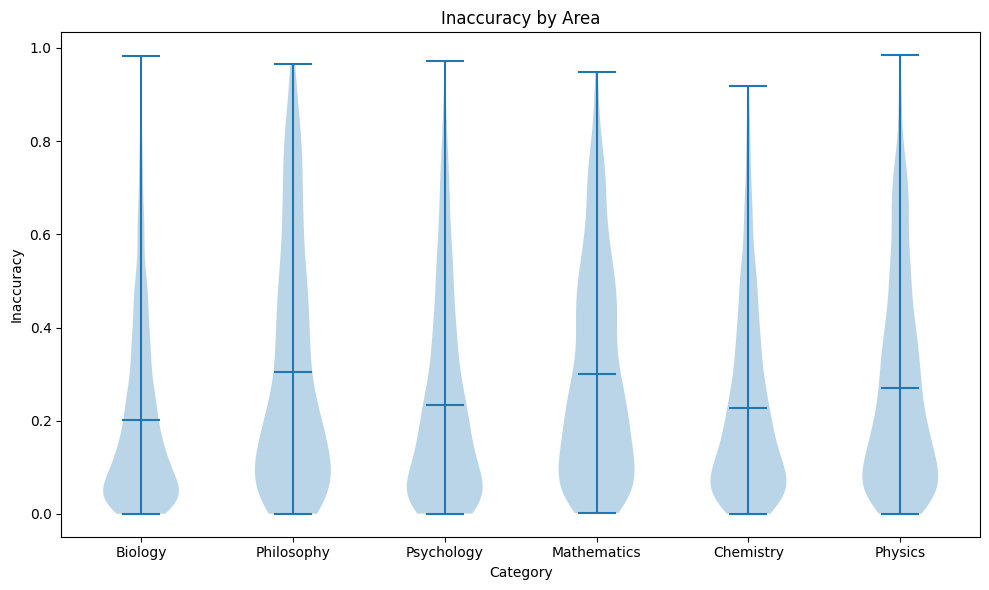
\includegraphics[scale=0.5]{inaccuracy_by_area}
\caption{\label{fig:inaccuracy-by-area}Inaccuracy by Area}
\end{figure}

Next, we estimated inaccuracy by looking at editorial debate rather than factual error (see Figure \ref{fig:inaccuracy-by-area}). We looked at each article’s talk page size and compared it to the total size of both the talk page and the article. A larger talk page means more discussion or disagreement. The violin plot shows that most articles in every field spend only a small part of their bytes on talk pages, but a few pages have much longer debates. In chemistry, most articles keep their talk pages below about 0.1 of the total bytes, and the median is just above that. Only a few articles reach up to 0.80. Biology, philosophy, and psychology also have most pages under roughly 0.15, but these fields have taller plots in the upper half. That means a few topics, like controversial medical issues in biology or big theoretical arguments in philosophy and psychology, spark long discussions. Mathematics and physics have the highest and widest range of debate. Their median sits around 0.25, and many pages go up to 0.5 or even 0.9, showing that some articles have as much discussion as main content. Overall, most scientific topics settle into low debate, but math and physics pages often have more back-and-forth about definitions, notation, and sources, while chemistry articles are more stable.

\begin{figure}[h]
\centering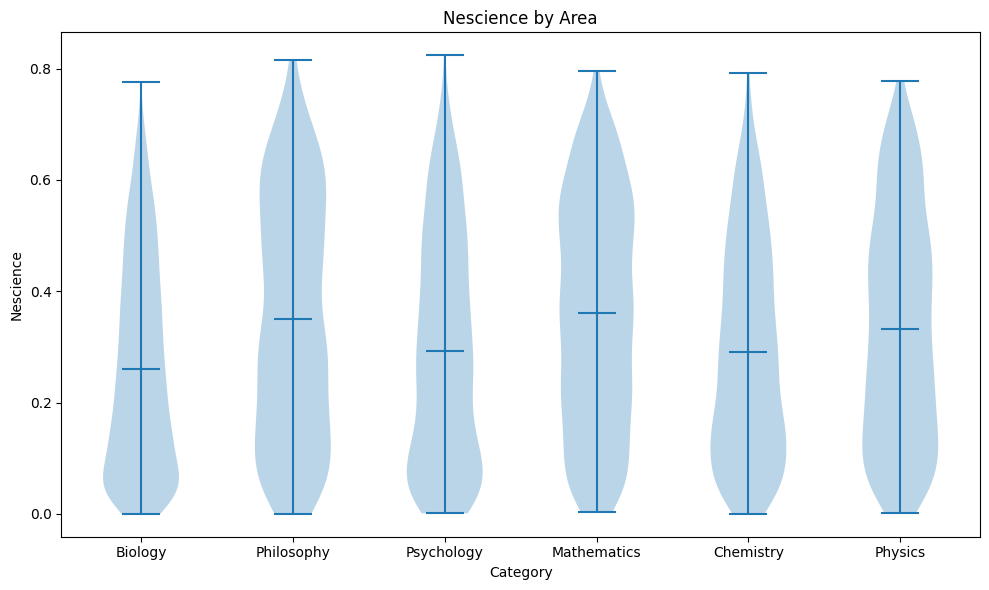
\includegraphics[scale=0.5]{nescience_by_area}
\caption{\label{fig:nescience-by-area}Nescience by Area}
\end{figure}

Finally, we combined redundancy and inaccuracy into one score, nescience (see Figure \ref{fig:nescience-by-area}). We first scaled each measure to range from 0 to 1, then took their harmonic mean. This score highlights pages that are either very repetitive, heavily debated, or both. In the violin plot, chemistry articles have low nescience (mostly under 0.20), showing they are concise and rarely debated. Biology is similar but has a few articles with higher scores, reflecting some ongoing talk-page discussions. Mathematics has the highest median nescience (around 0.40) and reaches up to 0.90, because many pages repeat concepts and have active debates over definitions. Philosophy and physics each show two peaks. one for well-settled articles near zero and one above 0.50 for more contested topics. Psychology mainly has low nescience, but some articles still face long debates. Overall, while every field has many well-covered pages, our nescience score shows that gaps in knowledge are biggest in mathematics and, to a lesser degree, in philosophy, physics, and psychology.

\begin{table}
\begin{centering}
\begin{tabular}{|c|c|c|c|}
\hline 
Category & Inaccuracy & Redundancy & Nescience \tabularnewline
\hline 
\hline
Biology & 0.157773 & 0.736704 & 0.229765 \tabularnewline
\hline
Chemistry & 0.122821 & 0.719500 & 0.183116 \tabularnewline
\hline
Mathematics & 0.271307 & 0.714365 & 0.392008 \tabularnewline
\hline
Philosophy & 0.144690 & 0.750007 & 0.244622 \tabularnewline
\hline
Physics & 0.223447 & 0.735314 & 0.297802 \tabularnewline
\hline
Psychology & 0.207355 & 0.721208 & 0.237835 \tabularnewline
\hline
\end{tabular}
\par\end{centering}
\caption{\label{tab:average_metrics_by_area}Average metrics by area}
\end{table}

Table \ref{tab:average_metrics_by_area} shows the average scores for each discipline. The numbers show that redundancy is almost the same across all six fields, ranging from 0.71 to 0.75, but inaccuracy varies more than a factor of two, from 0.12 in chemistry to 0.27 in mathematics. Because redundancy stays nearly constant, the differences in the combined nescience score come mostly from inaccuracy. In other words, after removing repeated boilerplate, the writing style is similar across subjects; what really changes is how much editors discuss or disagree on the talk pages. For example, chemistry’s low inaccuracy (0.12) gives it the smallest nescience (0.18), even with average redundancy. In contrast, mathematics has the highest inaccuracy (0.27) and therefore the highest nescience (0.39), despite slightly lower redundancy. Physics and psychology have similar redundancy (around 0.72–0.74), but physics sees more talk-page debate (0.22 vs. 0.21), so its nescience is higher than psychology’s. Philosophy shows the highest redundancy (0.75) but only a medium nescience (0.24) because its talk pages are quieter. Overall, this table tells us that for high-quality articles, the main difference between fields is how much editors argue, not how the text is written.

Putting together the redundancy and inaccuracy measures gives a single nescience score. This shows that all fields have similar writing patterns, most high‑quality articles compress to about 70–80\% of their original length, but they differ in how much they spark online discussions. Chemistry and biology have the quietest talk pages, so they score lowest on nescience. Mathematics and physics have more debates, so they score highest, even though their writing density is similar. Philosophy and psychology fall in between. These gaps happen because each field has many settled articles and a smaller group that need more discussion. In short, Wikipedia’s top science articles are usually concise and well written, but the talk pages reveal where editors still disagree most. The biggest knowledge gaps remain in math topics heavy on definitions and in physics areas open to different interpretations.

%
% Section: The Evolution of Knowledge
%

\section{The Evolution of Knowledge}

Our understanding of a scientific topic typically improves through sustained research efforts over time, resulting in a reduction of the topic's nescience, our lack of knowledge. Specifically, this improvement occurs through reductions in redundancy (repeated, unnecessary information) and inaccuracy (incorrect or misleading information), without significant increases in either component offsetting these improvements. New explanatory frameworks may emerge from innovative theories, refinements of existing theories, or simplified models. Ideally, each successive explanation will become more concise and accurate, removing previously redundant details and errors. Occasionally, new descriptions may temporarily lengthen as additional factual information is incorporated, causing a temporary increase in nescience. Nevertheless, the overall trend in scientific research should consistently be a progressive decrease in nescience as our knowledge advances.

To demonstrate how our theory can be used to characterize the evolution of our understanding of a scientific topic, that is, how nescience decreases with time, we have selected three highly relevant research topics as illustrative examples: graphene, CRISPR, and deep learning. Graphene\index{Graphene} is a single layer of carbon atoms arranged in a two-dimensional honeycomb lattice, known for its exceptional strength, conductivity, and versatility. CRISPR (Clustered Regularly Interspaced Short Palindromic Repeats)\index{CRISPR} is a revolutionary gene-editing technology that allows for precise, targeted modifications to DNA. Deep learning\index{Deep learning} is a subset of machine learning based on artificial neural networks, enabling complex pattern recognition and predictive modeling. These topics were chosen for their scientific importance and the richness of their associated descriptions, allowing us to apply our methodology and illustrate its effectiveness.

Figure \ref{tab:evolution-graphene} illustrates the evolution over time of redundancy, inaccuracy, and nescience metrics for the topic of Graphene. Each point on the graph corresponds to the analysis of a cleaned-up version of the Wikipedia page at a specific point in time. The early history of the graphene article shows the classic growth-and-turmoil phase of a fast-moving research topic. Between 2005 and 2010 redundancy climbed from $\approx$ 0.5 to just over 0.7 as the page ballooned with additional sections, figures and repeated explanations, while inaccuracy, our proxy for debate, spiked above 0.5. That surge coincides with the period when graphene research exploded in the literature, patents, and the popular press, so editors were actively negotiating scope, terminology and sourcing. The high redundancy plus high inaccuracy pushed the nescience curve to its peak near 0.9 in 2009-2010, signalling that the encyclopaedia's coverage lagged behind the field's rapid advances.

A sharp inflection occurs in 2011. The talk-page ratio collapses almost to zero-likely because extensive discussion was archived or split into sub-pages after the article stabilised-driving inaccuracy, and therefore nescience, down to negligible levels. From that point on the page continues to lengthen: redundancy drifts upward into the 0.78-0.82 band as definitions, production methods and applications are reiterated for different audiences. Yet talk-page activity remains a small fraction of total bytes, so nescience stays close to zero with only minor blips when new findings (e.g., commercial production techniques around 2014 or 2019) briefly rekindle debate. The negative regression slope on both the inaccuracy and nescience plots confirms a long-term convergence toward consensus, while the positive slope on redundancy simply reflects a mature, template-rich article that keeps accumulating detail without reopening fundamental disputes.

\begin{table}
\begin{centering}
\begin{tabular}{|c|c|c|}
\hline 
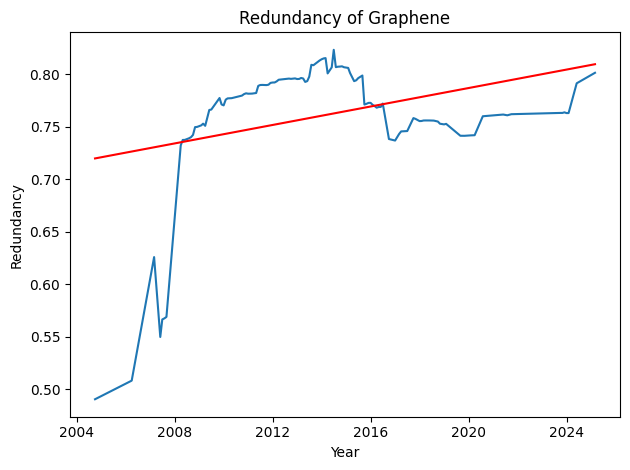
\includegraphics[width=0.3\textwidth]{redundancy_graphene}
&
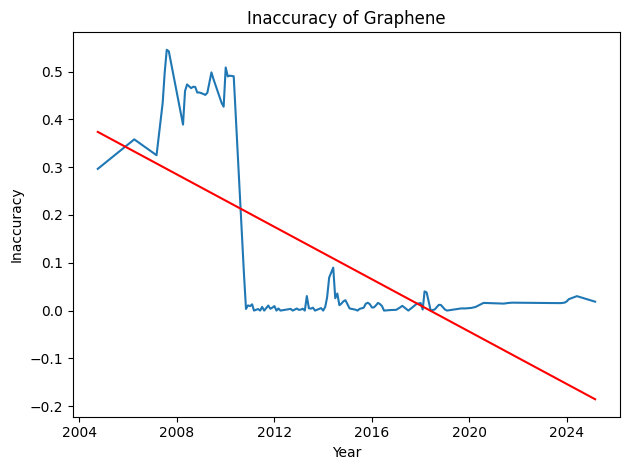
\includegraphics[width=0.3\textwidth]{inaccuracy_graphene}
&
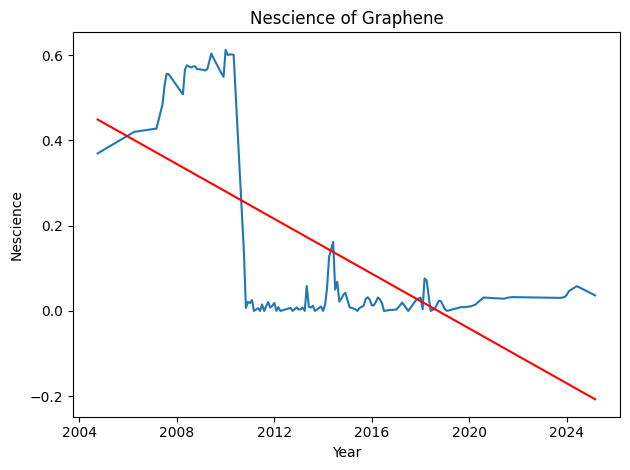
\includegraphics[width=0.3\textwidth]{nescience_graphene}\tabularnewline
\hline 
\end{tabular}
\par\end{centering}
\caption{\label{tab:evolution-graphene}Knowledge evolution of graphene}
\end{table}

CRISPR's Wikipedia trajectory (see Figure \ref{tab:evolution-CRISPR}) mirrors the arc of a scientific whirlwind maturing into mainstream knowledge. When the page first took shape (2010 - 2013) redundancy sat in the low-to-mid 0.60, reflecting a compact article that still compressed poorly, while inaccuracy-driven by an energetic talk page-hovered around 0.40. Those years coincide with the burst of laboratory discoveries that turned CRISPR-Cas9 from an obscure bacterial defence into a headline-making gene-editing tool, so editors were constantly renegotiating scope and sourcing. Both factors pushed nescience above 0.70, signalling a large knowledge gap between fast-moving science and the encyclopaedia's ability to consolidate it.

A decisive shift occurs in 2015-2016. The talk-page share collapses, dropping inaccuracy to near zero almost overnight; the page was substantially rewritten and much of the debate was archived once standard terminology, mechanism diagrams and milestone experiments had stabilised. Redundancy, meanwhile, jumps above 0.75 and keeps inching up as new sections on ethics, patents and clinical trials are added-material that inevitably repeats the core biology and acronyms. With one input shrinking and the other growing only slowly, nescience plummets and stays near the floor, apart from brief spikes that map neatly onto external flashpoints (the 2018 gene-edited-babies scandal, for example).

The overall downward regression slopes for both inaccuracy and nescience confirm a steady convergence toward consensus, while the upward slope in redundancy simply records the article's swelling, template-rich structure. By 2020 the CRISPR page looks much like that of graphene in its mature phase: highly compressible, rarely contested, and updated incrementally rather than rewritten from scratch each time the field advances.

\begin{table}
\begin{centering}
\begin{tabular}{|c|c|c|}
\hline 
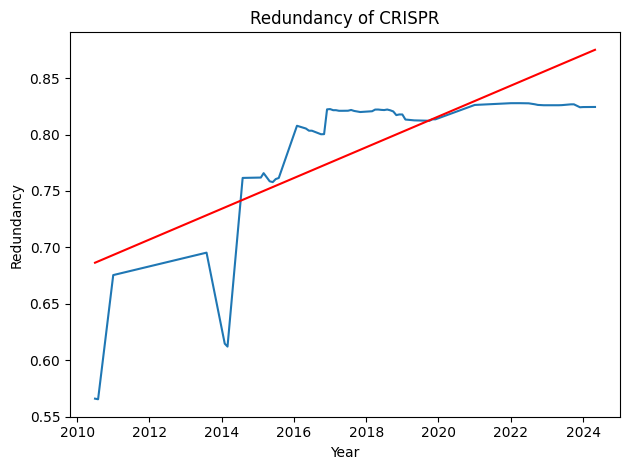
\includegraphics[width=0.3\textwidth]{redundancy_CRISPR}
&
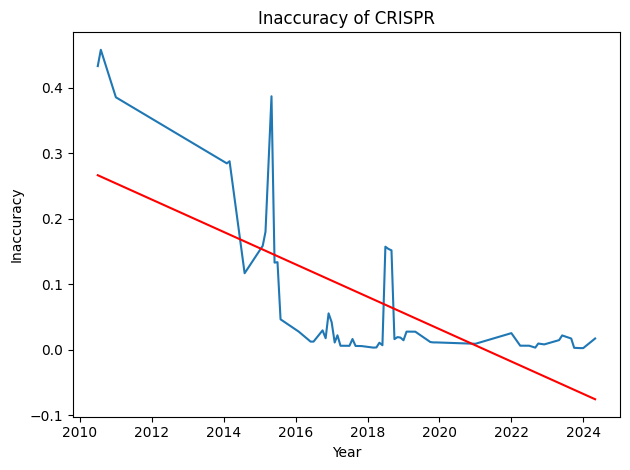
\includegraphics[width=0.3\textwidth]{inaccuracy_CRISPR}
&
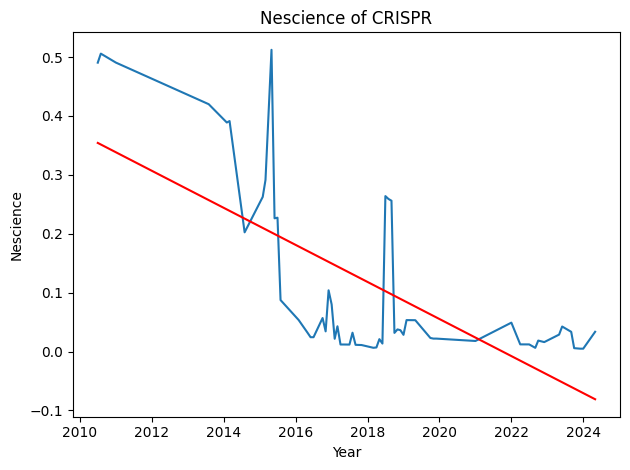
\includegraphics[width=0.3\textwidth]{nescience_CRISPR}\tabularnewline
\hline 
\end{tabular}
\par\end{centering}
\caption{\label{tab:evolution-CRISPR}Knowledge evolution of CRISPR}
\end{table}

The deep-learning article (see \ref{tab:evolution-deep-learning}) traces a pattern typical of a field that shifted from niche research to global headline status almost overnight. In its early years (2011-2014) the page was compact and still being drafted: redundancy climbed from  $\approx$ 0.40 to the low 0.70 as basic definitions, algorithm lists and seminal breakthroughs were added and often restated, while inaccuracy oscillated but stayed below 0.30, reflecting moderate talk-page traffic. The real turbulence began in 2017: the talk-page share abruptly jumped above 0.40 and stayed there for nearly five years, mirroring the community's debates over benchmark claims, ethics, and the hype surrounding "AI booms." Because redundancy had already settled in the mid-0.70s, this burst of discussion drove nescience to a sustained plateau above 0.85, marking the article as one of Wikipedia's most actively contested science pages during the height of deep-learning publicity.

A dramatic correction occurs in late 2022. Large chunks of deliberation were apparently archived or spun off, slashing inaccuracy to near zero almost overnight and dropping nescience with it. Since then the page has remained highly compressible (redundancy $\approx$ 0.75 - 0.78) but largely uncontested; only small upticks appear as new foundation-model milestones are folded in. The negative regression slopes for inaccuracy and nescience therefore chart a long-run movement toward consensus, even though the five-year plateau of high nescience serves as a reminder that Wikipedia's knowledge gap can stay wide for a protracted period when a discipline's methods, jargon and social implications are evolving faster than editors can lock down a stable narrative.

\begin{table}
\begin{centering}
\begin{tabular}{|c|c|c|}
\hline 
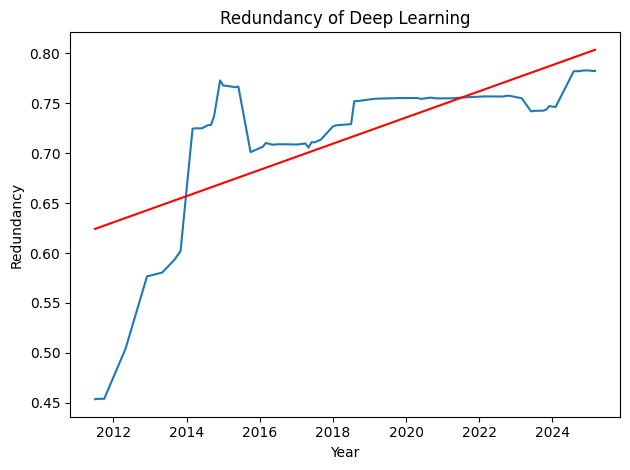
\includegraphics[width=0.3\textwidth]{redundancy_deep_learning}
&
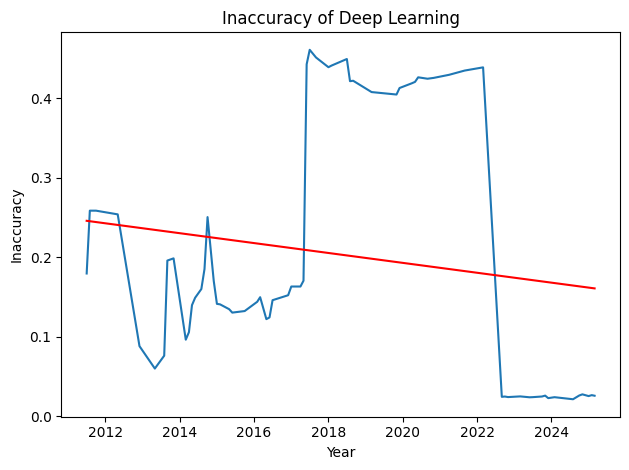
\includegraphics[width=0.3\textwidth]{inaccuracy_deep_learning}
&
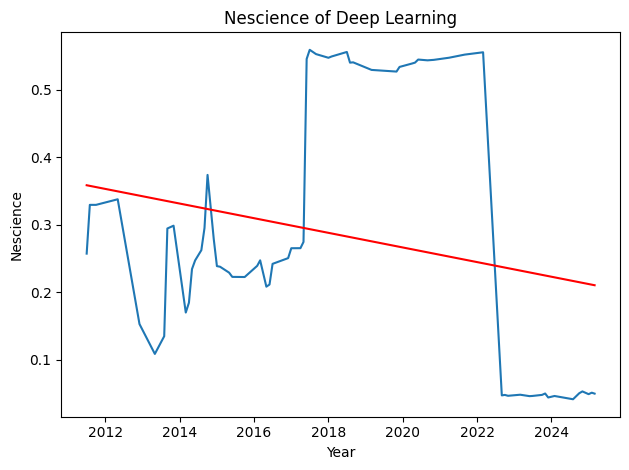
\includegraphics[width=0.3\textwidth]{nescience_deep_learning}\tabularnewline
\hline 
\end{tabular}
\par\end{centering}
\caption{\label{tab:evolution-deep-learning}Knowledge evolution of deep learning}
\end{table}

Across three emblematic case studies (graphene, CRISPR and deep learning) the time-series confirm that Wikipedia's nescience reliably chronicles the lifecycle of a scientific topic: initial growth brings a surge of redundancy as material is layered on, and a spike of inaccuracy as editors negotiate scope and sourcing; once consensus forms, talk-page activity collapses, redundancy stabilises in the high-0.70s, and nescience falls toward zero.  Graphene reached this mature phase around 2011, CRISPR around 2016, while deep learning lingered in a high-gap state from 2017 to 2022 before a mass archiving of debate produced an abrupt convergence. The trajectory is thus quantifiable: rising redundancy without rising inaccuracy signals steady accretion of detail, whereas persistent high nescience marks periods when the science itself, or its social framing, is still in flux.

%
% Section: The Demarcation Problem
%
\section{The Demarcation Problem}

In this section, we propose a practical method, based on the theory of nescience, to address the demarcation problem\index{Demarcation problem}, specifically, the challenge of distinguishing scientific from non-scientific knowledge in real-world contexts. Although demarcation is a longstanding philosophical issue, our aim is not to conclusively solve this complex problem but rather to provide insights into its nature and outline potential paths toward future solutions through practical and operational methods.

For our experiments and analysis, we have selected six scientific topics and six pseudoscientific topics to evaluate our approach to the demarcation problem. Our analysis is based on the descriptions of these topics provided by Wikipedia and their associated \texttt{Talk} pages. As in previous analyses conducted in this chapter, we have preprocessed the Wikipedia pages by using the \texttt{wikitextparser} Python library to remove Wikimedia tags and other irrelevant elements such as tables and images.

The six scientific topics selected are: Climate Change (the long-term alteration of temperature and weather patterns), Graphene (a single-layer carbon material with extraordinary physical properties), Dark Matter (a hypothesized form of matter making up approximately 85\% of the universe), Deep Learning (a subset of machine learning using neural networks with multiple layers), Lithium-ion Battery (a type of rechargeable battery widely used for portable electronics and electric vehicles), and Brain-Computer Interface (a technology enabling direct communication between the brain and external devices). These scientific topics have been selected due to their intensive research activity over the past 20 years.

\begin{figure}[H]
\centering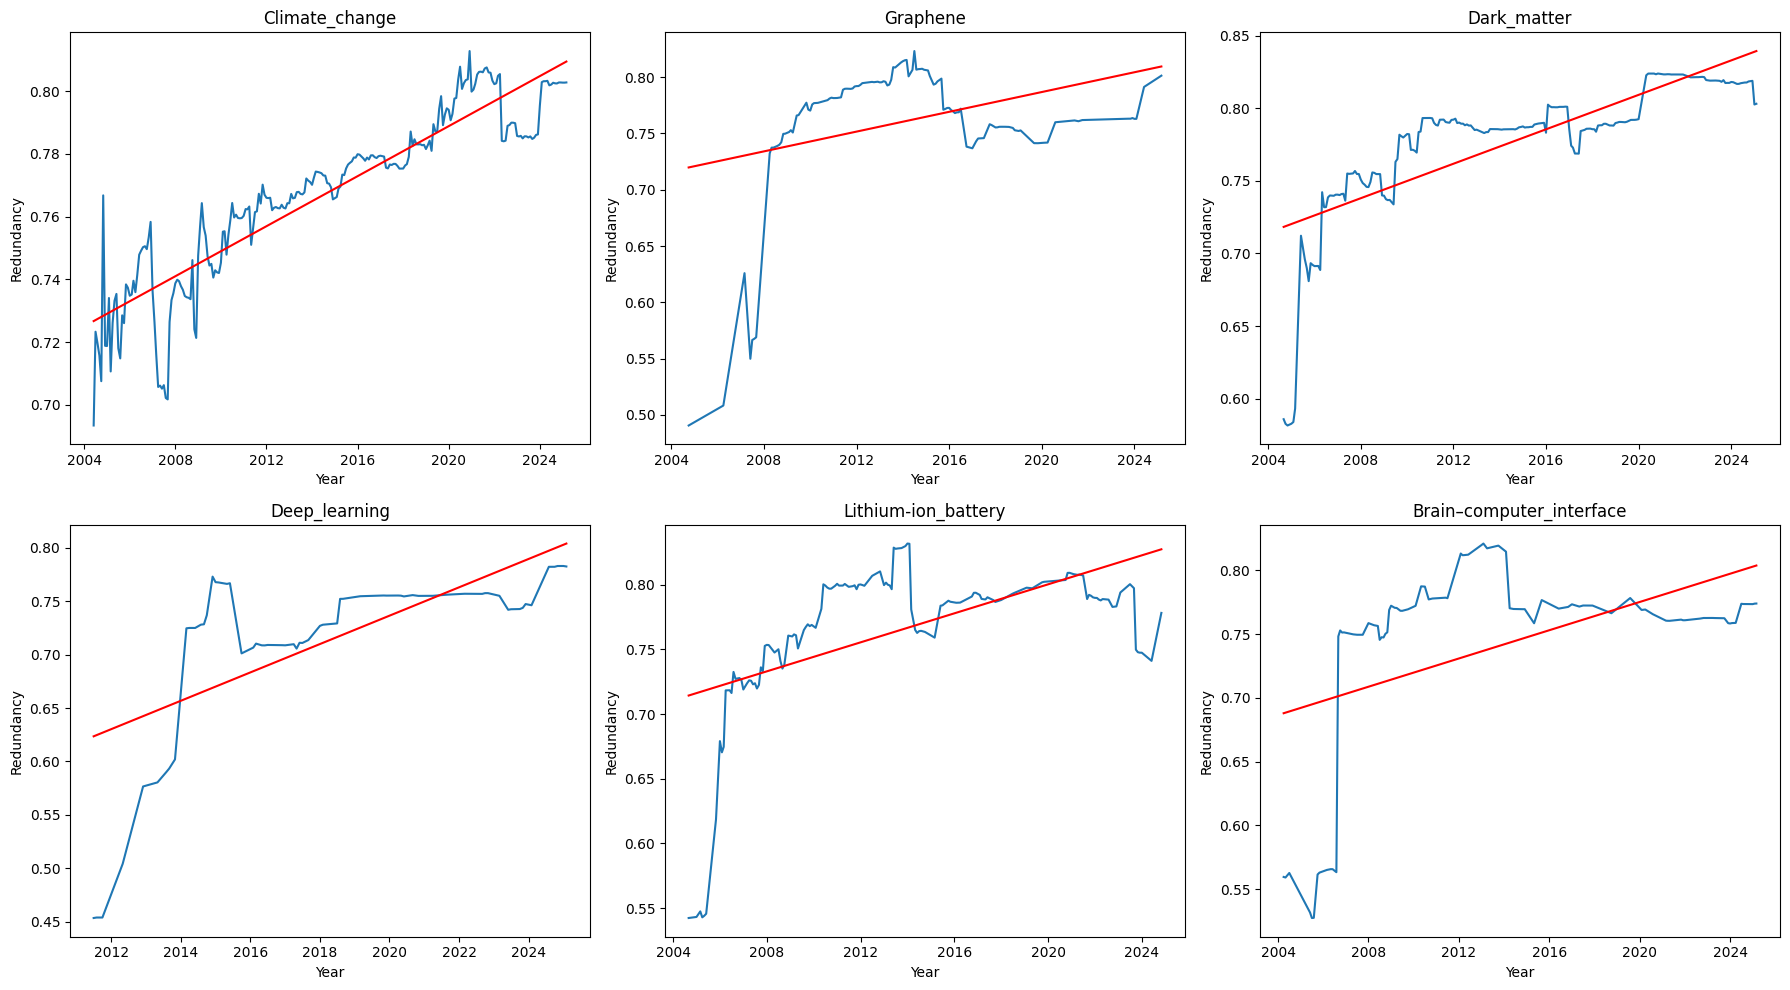
\includegraphics[scale=0.3]{RedundancySixScientific}
\caption{\label{fig:redundancy_six_scientific}Evolution of Redundancy in Scientific Topics}
\end{figure}

Redundancy, as an approximation of the concept of surfeit, is computed, as in the previous case, by comparing the ratio of the length of a text to its compressed version. Figure \ref{fig:redundancy_six_scientific} shows the evolution of redundancy for these selected scientific topics over the past 20 years. As observed, redundancy for these topics demonstrates an increasing trend, as confirmed by the computed regression line. Although one might generally expect redundancy to decrease as our understanding improves, new discoveries and emerging knowledge frequently necessitate additional details and explanations, thus increasing redundancy in descriptions.

\begin{figure}[H]
\centering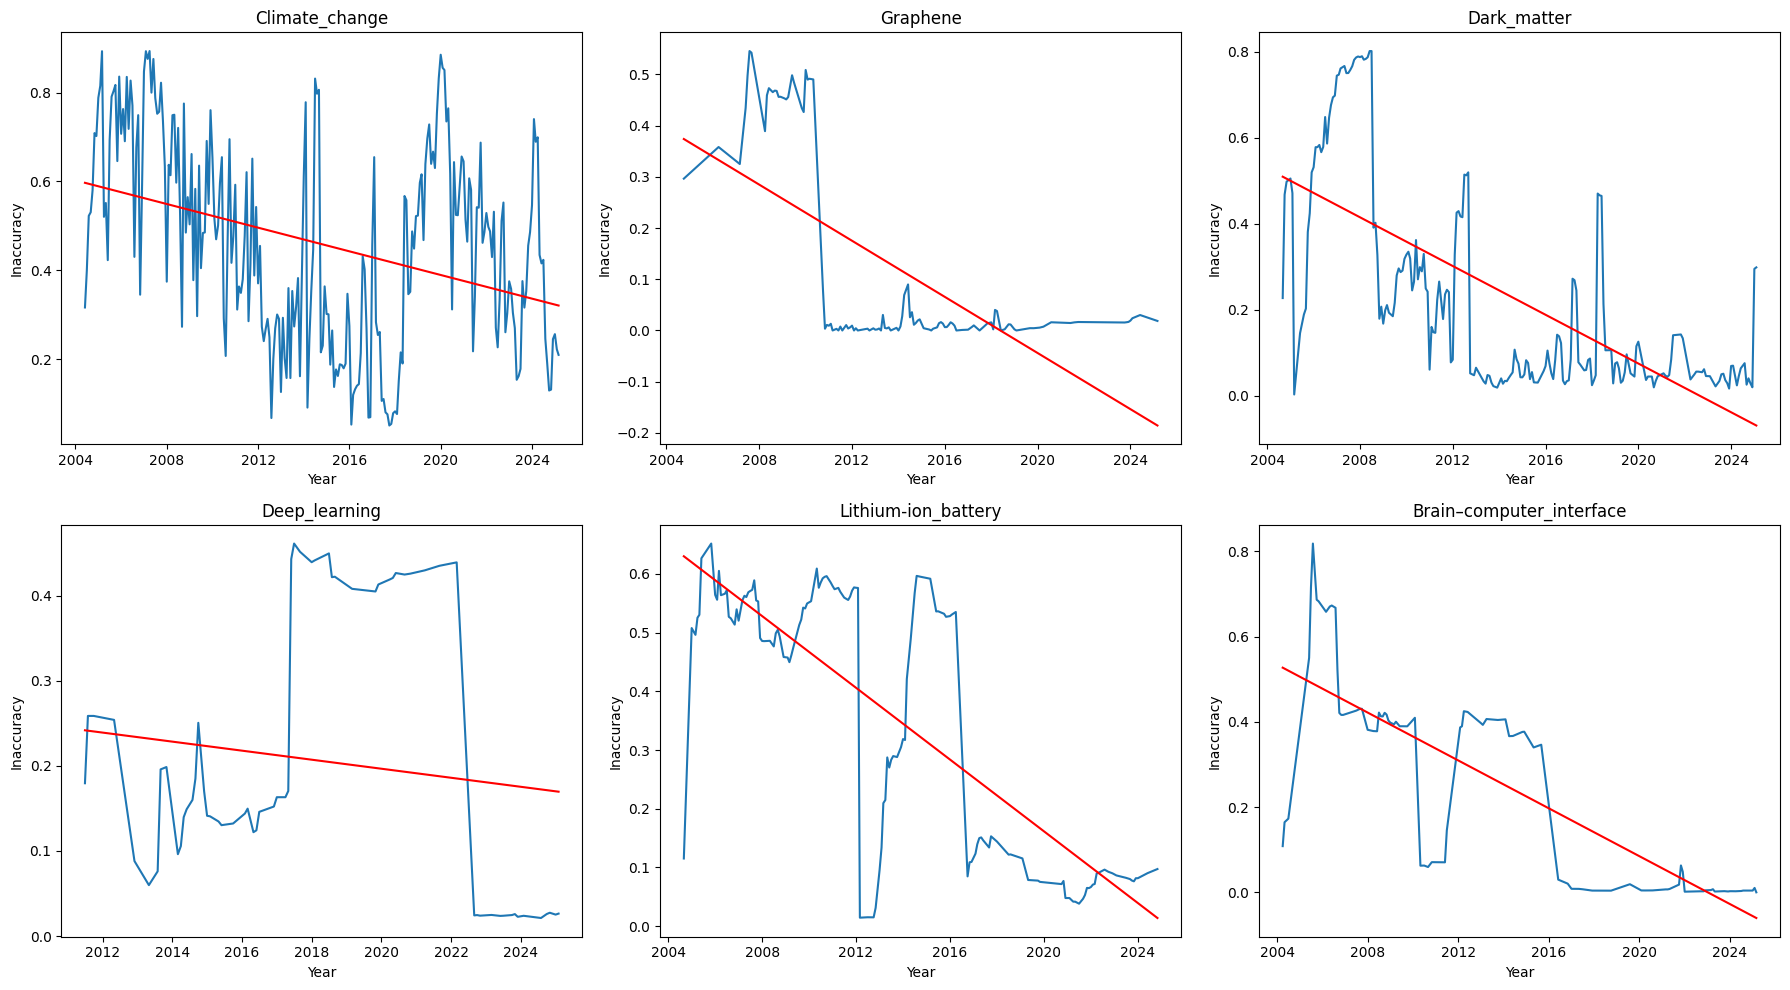
\includegraphics[scale=0.3]{InaccuracySixScientific}
\caption{\label{fig:inaccuracy_six_scientific}Evolution of Inaccuracy in Scientific Topics}
\end{figure}

Inaccuracy is computed based on the ratio length\_talk / (length\_talk + length\_article), where length\_talk represents the length of the Talk page for each topic, and length\_article is the length of the corresponding Wikipedia article, as done in the previous sections. Utilizing Talk pages is an effective method for approximating article inaccuracy since these pages typically contain discussions, disputes, and clarifications regarding inaccuracies or controversies in the articles. Figure \ref{fig:inaccuracy_six_scientific} illustrates the evolution of inaccuracies for the selected scientific topics, showing a clear decreasing trend across all topics.

\begin{figure}[H]
\centering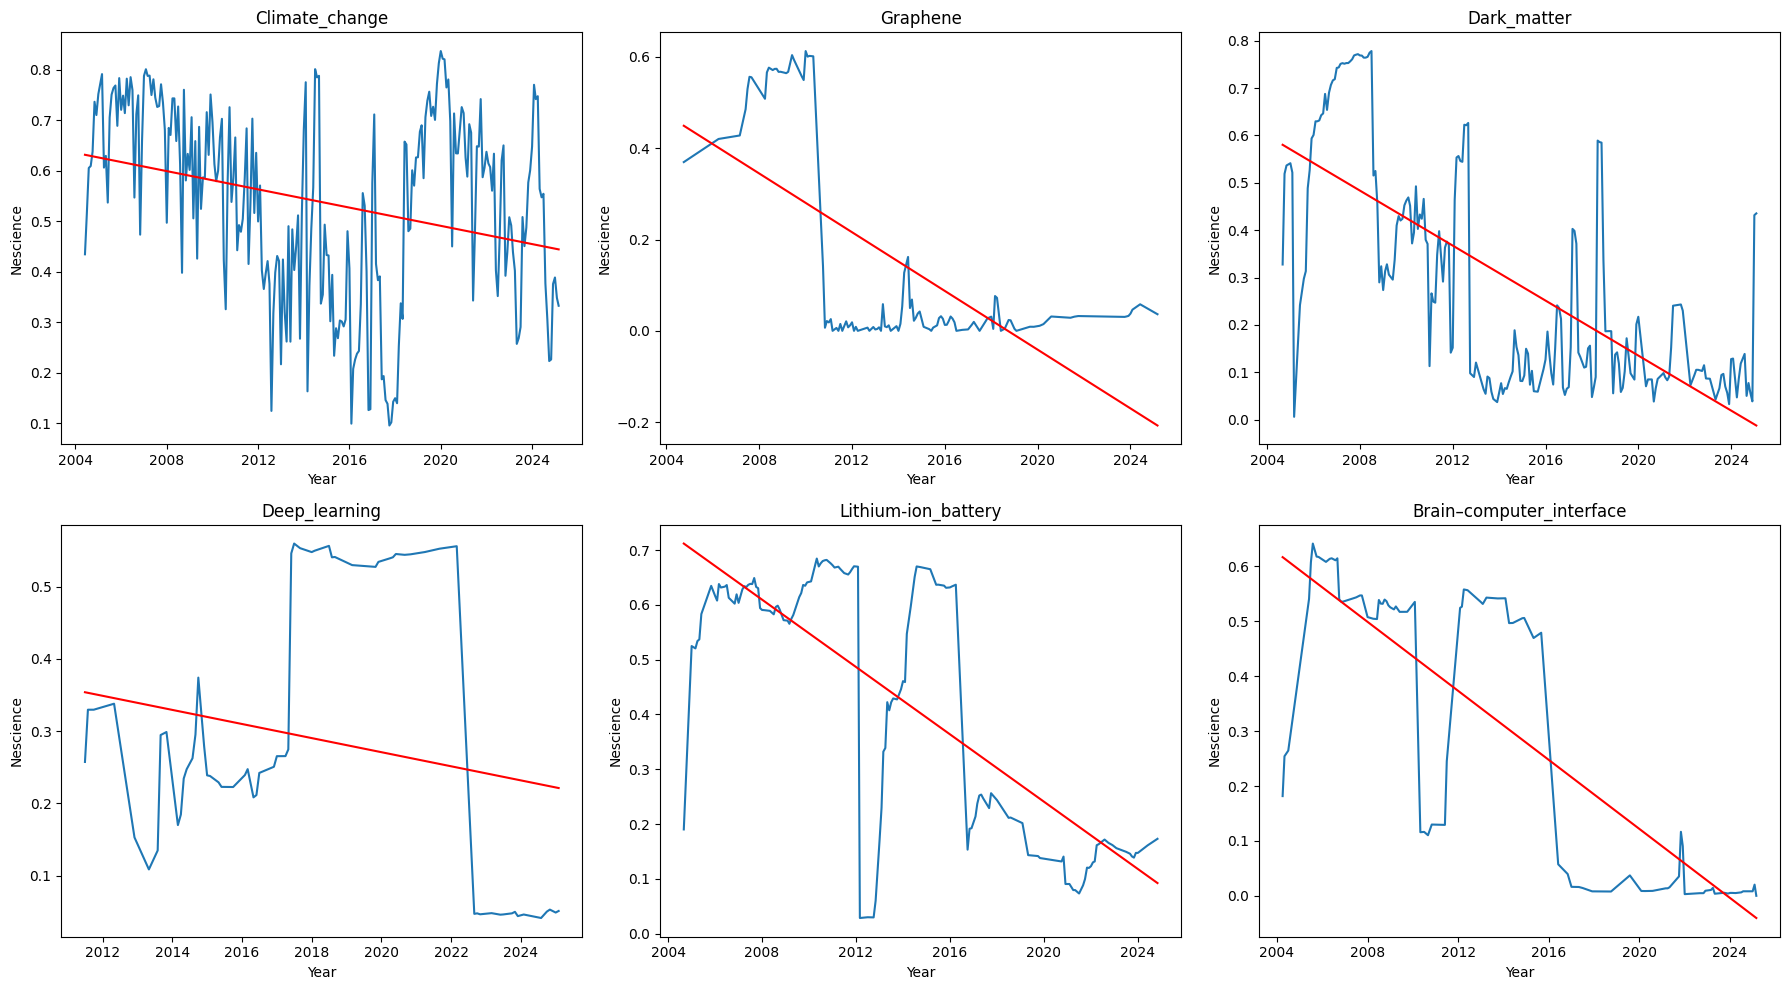
\includegraphics[scale=0.3]{NescienceSixScientific}
\caption{\label{fig:nescience_six_scientific}Evolution of Nescience in Scientific Topics}
\end{figure}

Finally, Figure \ref{fig:nescience_six_scientific} shows the evolution of nescience for all selected scientific topics, where nescience is estimated as the harmonic mean of the metrics of redundancy and inaccuracy. As depicted, despite the positive trend in redundancy, nescience exhibits a decreasing trend, suggesting our overall understanding of these topics improves over time.

Additionally, we have selected six pseudoscientific topics to further evaluate our demarcation method: Lunar Effect (the belief that lunar cycles influence human behavior), Water Memory (the claim that water retains a memory of substances previously dissolved in it), Astral Projection (the claimed ability of consciousness to leave the physical body and travel in the astral plane), Enneagram of Personality (a model describing personality types based on a geometric figure with nine interconnected points), Perpetual Motion (the hypothetical concept of a machine that operates indefinitely without energy input), and Dowsing (a technique claiming the ability to locate water, minerals, or other hidden substances through intuitive means). These topics represent different pseudoscientific categories—Lunar Effect (Astrology), Water Memory (Homeopathy), Astral Projection (Parapsychology), Enneagram of Personality (Numerology), Perpetual Motion (Physics-related pseudoscience), and Dowsing (Divination)—and were selected based on classifications from Wikipedia itself as pseudoscience.

\begin{figure}[H]
\centering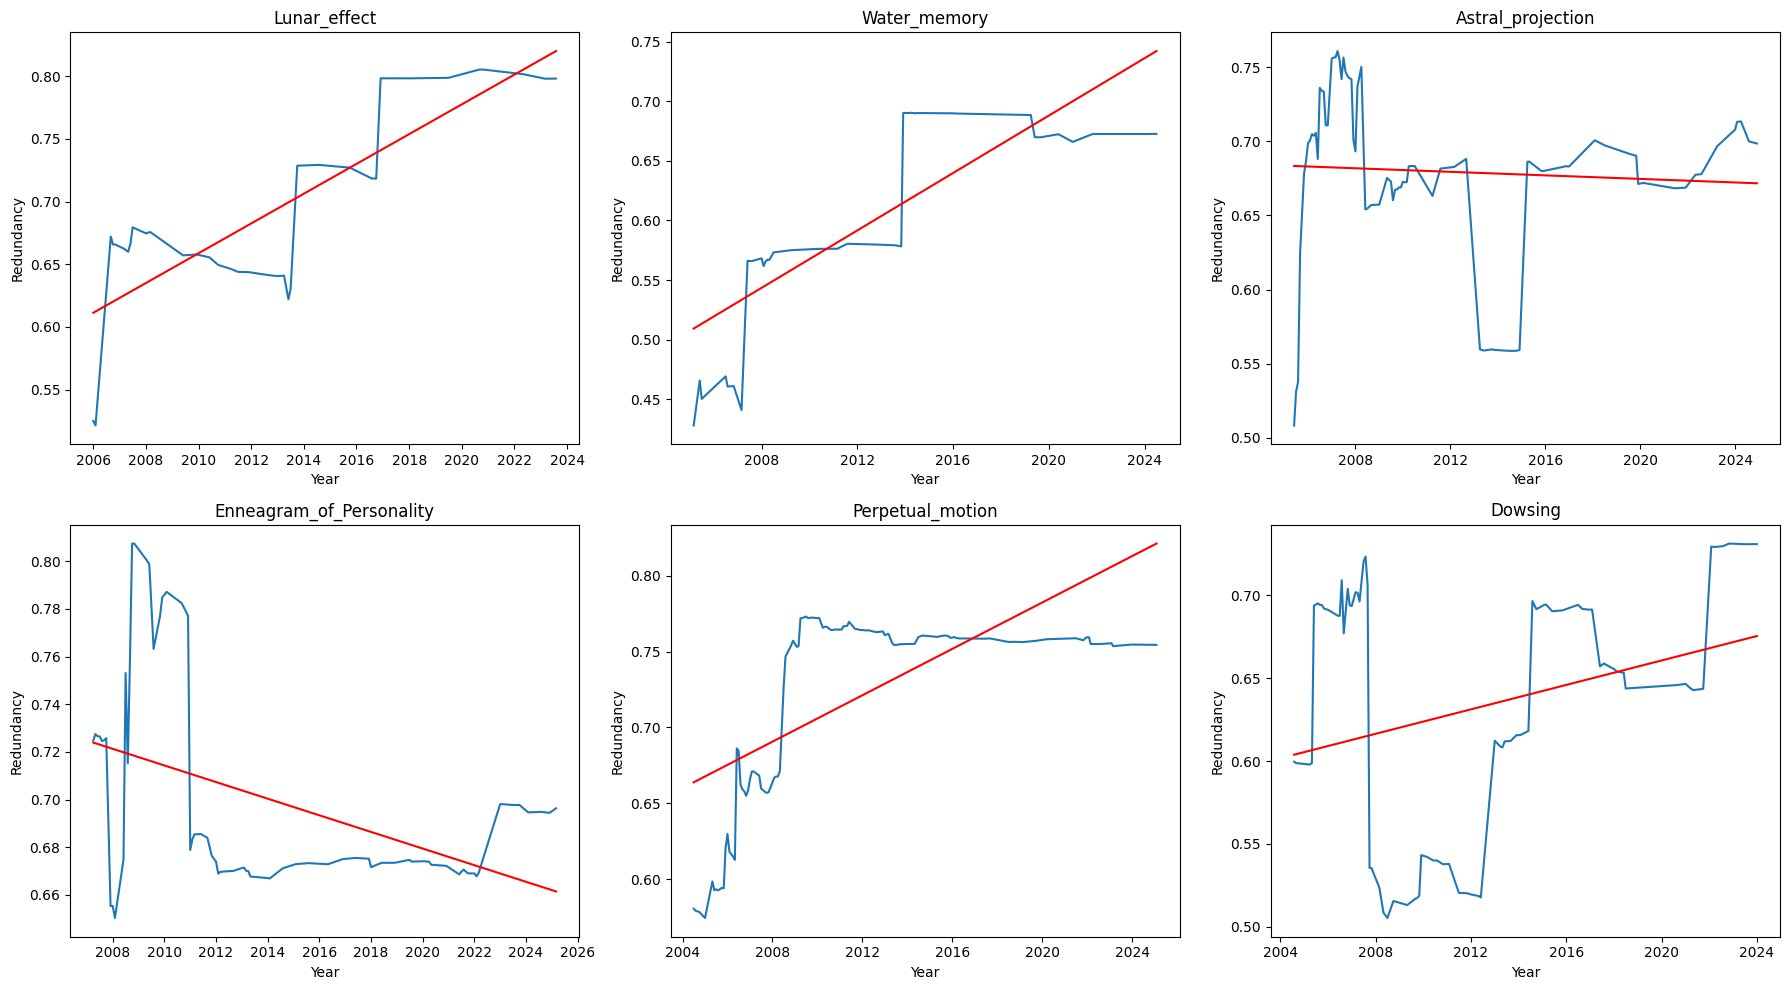
\includegraphics[scale=0.3]{RedundancySixPseudoscientific}
\caption{\label{fig:redundancy_six_pseudoscientific}Evolution of Redundancy in Pseudoscientific Topics}
\end{figure}

Figure \ref{fig:redundancy_six_pseudoscientific} shows the evolution of redundancy for these selected pseudoscientific topics over the past 20 years. As it was the case of scientific topics, redundancy for these topics demonstrates an increasing trend for "Lunar Effect", "Water Memory", "Perpetual Motion", and "Dowsing", and a rather surprising non-increasing trend for "Astral Projection" and "Enneagram of Personality". This decrease in redundancy for the latter two topics may indicate that their Wikipedia articles have undergone substantial editing aimed at streamlining or simplifying the content.

\begin{figure}[H]
\centering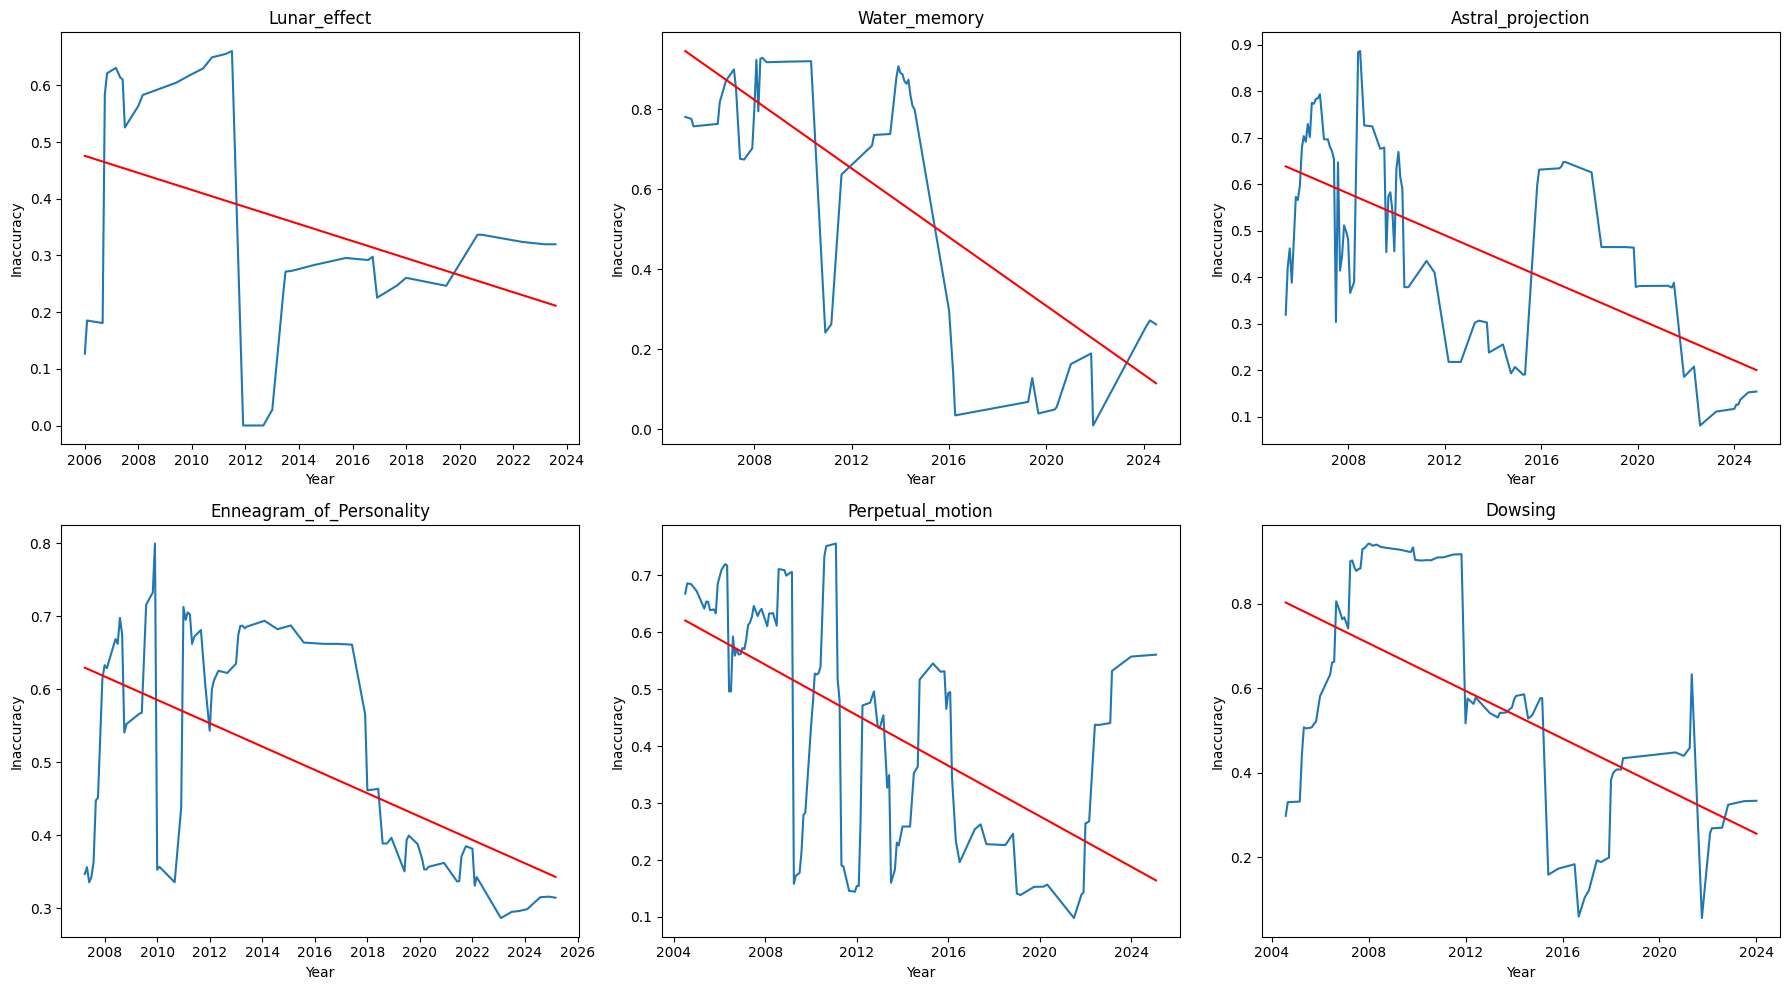
\includegraphics[scale=0.3]{InaccuracySixPseudoscientific}
\caption{\label{fig:inaccuracy_six_pseudoscientific}Evolution of Inaccuracy in Pseudoscientific Topics}
\end{figure}

Figure \ref{fig:inaccuracy_six_pseudoscientific} illustrates the evolution of the estimated inaccuracies for the same pseudoscientific topics. A clear decreasing trend in inaccuracies is observable across most topics, suggesting, somewhat unexpectedly, that controversies regarding these topics have started to settle down. 

\begin{figure}[H]
\centering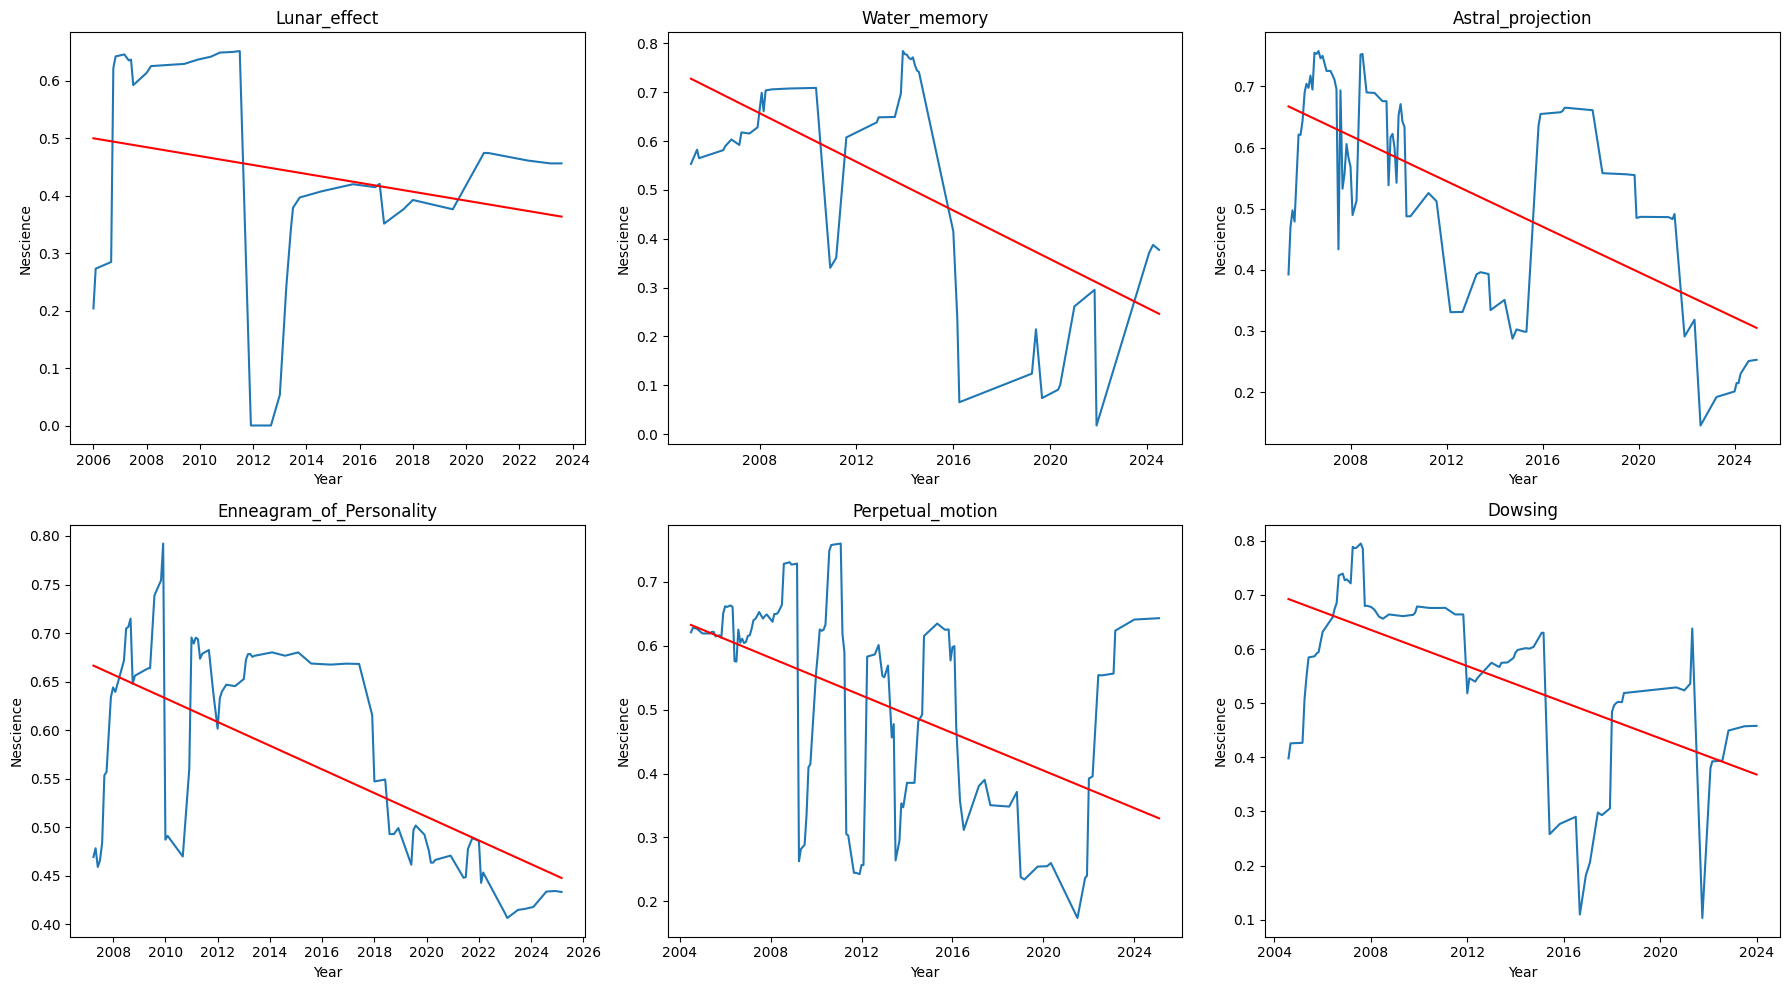
\includegraphics[scale=0.3]{NescienceSixPseudoscientific}
\caption{\label{fig:nescience_six_pseudoscientific}Evolution of Nescience in Pseudoscientific Topics}
\end{figure}

Finally, Figure \ref{fig:nescience_six_pseudoscientific} shows the evolution of the estimated nescience for all selected pseudoscientific topics. As expected, given the previous figures for redundancy and inaccuracy, a decreasing trend is observed for most topics, suggesting that our knowledge about this topics has, in fact, decreased with time.

Our preliminary analysis is too superficial to draw definitive conclusions. A more detailed analysis, employing randomized controlled experiments and rigorous hypothesis testing, needs to be conducted. Additionally, the approximations for redundancy and inaccuracy could be refined further (e.g., citation analysis, scientific community surveys, bibliometric analysis). Based on our initial findings, there appear to be no significant practical differences between science and pseudoscience—both communities seem capable of increasing our knowledge about their respective topics. The essential distinction between science and pseudoscience may lie in the validity and truthfulness of claims, rather than in their methodologies. Alternatively, demarcation could also be based on science's demonstrated capability to transform theoretical results into practical, real-world applications—a capability generally lacking in pseudoscience.

%
% Section: Perfect Knowledge
%
\section{Perfect knowledge}

Philosophers of science deal with the problem of how knowledge about our world is gathered trough our senses, and if we can trust our perceptions. Also, they address the difficult issue of how knowledge is derived from facts (for example, by means of applying the principle of induction), and if it is sound, from a logic point of view, to make those derivations. Finally, philosophers are interested in how scientific theories are generated based in this knowledge. Any of these problems is covered by the theory of nescience, since we assume that theories (or descriptions in our own terminology) are already known. We do not provide any method to create those theories. What the theory of nescience provides is a set of metrics to quantitatively evaluate, and compare, existing scientific theories. 

It might appear that the descriptions in which the theory of nescience is based are truly objective, in the sense that they must be so clear and well stated that even a computer can reconstruct the original topic given its description. Although this point is true, the problem that prevents the theory to provide an absolute knowledge about our world is the way we choose the entities to study, and how we encode as strings those entities. As we have seen (see Chapter \ref{cha:Topics-and-Descriptions}), the accuracy of our descriptions depend on how good is our encoding of the abstract entities we are studying. Unless the entities are strings themselves, we must assume that our encoding could not be perfect. Moreover, we could be wrong about our assumption that the selected set of entities covers all possible entities of that kind. That is, the set of entities are subject to change as our scientific understanding about them develops. {\color{red} The same might happen in case of encodings.}

Although the theory of nescience does not say anything about how we can reach an absolute knowledge about an entity, it can tell us if we have reached a perfect description (that we make equal to a perfect knowledge). That is, the theory of nescience can answer the question if we have reached a perfect knowledge about a topic, subject that the the entity under study has been properly identified, and the encoding of this entity has no errors.

%
% Section: Unknown Unknown
%
\section{Uknown-unknown}



%
% Section: References
%
\section*{References}

{\color{red} Provide a reference to Wikpedia}

The behavior of compressors depending of the size of objects and window (buffer) size is studied in detail in \cite{cebrian2005common} with applications to the normalized compression distance (a measure of similarity between objects proposed in \cite{li2004similarity}).

Add a reference to the Burrows–Wheeler algorithm and to bzip2, and gzip. Perhaps a comparison, or more bib in NCD in practice.

% **CRISPR**
% 
% 1. Doudna, J. A. & Charpentier, E. “The new frontier of genome engineering with CRISPR‑Cas9,” *Science* 346, 1258096 (2014). ([Science][1])
% 2. Barrangou, R. & Doudna, J. A. “Applications of CRISPR technologies in research and beyond,” *Nature Biotechnology* 34, 933–941 (2016). ([Nature][2])
% 
% These two papers trace the jump from the basic molecular mechanism to the first broad survey of practical uses, neatly bracketing CRISPR’s move from discovery to applied tool‑set.
%
% ---
% 
% **Graphene**
% 
% 1. Novoselov, K. S. *et al.* “Electric field effect in atomically thin carbon films,” *Science* 306, 666–669 (2004). ([Science][3])
% 2. Castro Neto, A. H., Guinea, F., Peres, N. M. R., Novoselov, K. S. & Geim, A. K. “The electronic properties of graphene,” *Reviews of Modern Physics* 81, 109–162 (2009). ([Physical Review][4])
% 
% Together these references cover the first experimental isolation of graphene and a comprehensive review of its physics just five years later.
% 
% ---
% 
% **Deep learning**
% 
% 1. LeCun, Y., Bengio, Y. & Hinton, G. “Deep learning,” *Nature* 521, 436–444 (2015). ([Nature][5])
% 2. Schmidhuber, J. “Deep learning in neural networks: an overview,” *Neural Networks* 61, 85–117 (2015). ([ScienceDirect][6])
% 
% The Nature article presents the field’s modern milestones and outlook, while Schmidhuber’s survey places those achievements in the longer historical context of neural‑network research.
% 
% [1]: https://www.science.org/doi/10.1126/science.1258096?utm_source=chatgpt.com "The new frontier of genome engineering with CRISPR-Cas9 - Science"
% [2]: https://www.nature.com/articles/nbt.3659?utm_source=chatgpt.com "Applications of CRISPR technologies in research and beyond - Nature"
% [3]: https://www.science.org/doi/10.1126/science.1102896?utm_source=chatgpt.com "Electric Field Effect in Atomically Thin Carbon Films - Science"
% [4]: https://link.aps.org/doi/10.1103/RevModPhys.81.109?utm_source=chatgpt.com "The electronic properties of graphene | Rev. Mod. Phys."
% [5]: https://www.nature.com/articles/nature14539?utm_source=chatgpt.com "Deep learning - Nature"
% [6]: https://www.sciencedirect.com/science/article/pii/S0893608014002135?utm_source=chatgpt.com "Deep learning in neural networks: An overview - ScienceDirect.com"



